\chapter{Digital pathology}
\label{chap:backdp}

\begin{overview}{Overview}
  This chapter presents an overview of digital and \acrlong{cpath} from the perspective of a computer scientist and aims at providing basic understanding of what makes \acrlong{cpath} a challenging but promising topic. Section \ref{sec:backdp:wsi} presents a typical histological glass slide preparation procedure, how this glass slide is transformed into an image and what could go wrong during the process. Section \ref{sec:backdp:typicalanalysistasks} discusses briefly how slides are used and analyzed by practioners and provides three use cases where \acrlong{cpath} could greatly help pathologists in their day-to-day work. Finally, in Section \ref{sec:backdp:ml}, we present some of the challenges specific to the application of machine learning to \acrlong{cpath} including data leakage and data scarcity and how to tackle them. This last section also presents the related works of our contributions.
\end{overview}

% analogintelligence.com image dp illustration

\section{What is \acrlong{dp}?}
\label{sec:backdp:whatisdp}

Nowadays, medicine and healthcare rely heavily on analysis of body samples to study and diagnose diseases. The branch of medicine focusing on this analysis is called \textit{pathology} which includes histology-based pathology and cytology-based pathology (\aka histopathology and cytopathology respectively). Both of these sub-branches involve the study of microscope glass slides containing samples (see Figure \ref{fig:backdp:glassslides}). Histology samples are tissue sections cut from a bodily specimen. Cytology is concerned with samples of free cells or tissue fragments.

\begin{figure}
  \centering
  \begin{subfigure}[t]{0.48\textwidth}
    \centering
    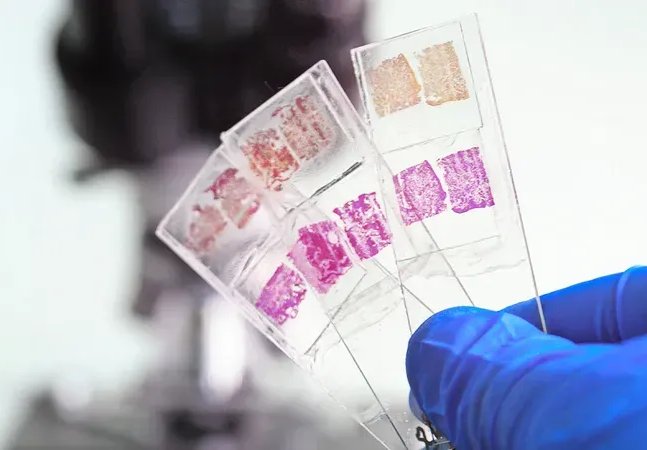
\includegraphics[height=150pt]{backdp/microscope-slide.png}
  \end{subfigure}
  \begin{subfigure}[t]{0.48\textwidth}
    \centering
    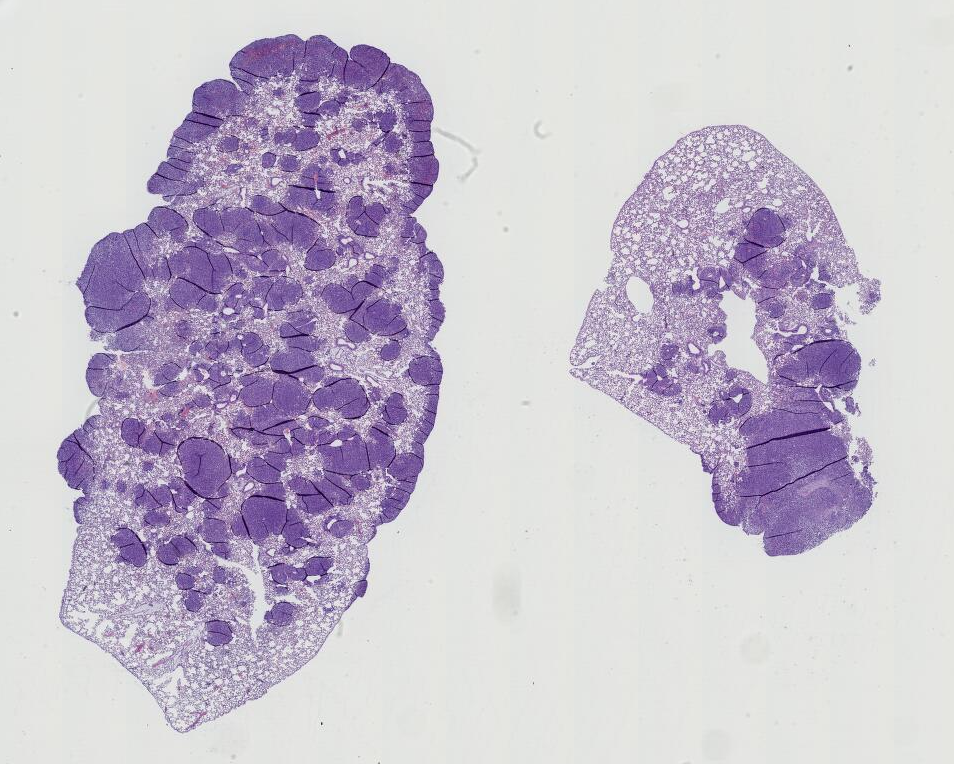
\includegraphics[height=150pt]{backdp/wsi.png}
  \end{subfigure}
  \caption{\textit{Left:} microscope slides with tissue samples (source: \cite{img:glassslides}). \textit{Right:} a whole-slide image of dimensions 30720 x 25600 pixels.}
  \label{fig:backdp:glassslides}
\end{figure}

The trend of digitalization affecting our societies also impacts pathology as, using dedicated scanners, a glass slide can now be digitized into large image file called a \acrfirstit{wsi}. These files associated with subject metadata are stored in computer systems commonly called \acrfirst{pacs} or \acrfirst{lis}. In this context, \acrfirstit{dp} can be defined as ``\textit{the acquisition, management, sharing and interpretation of pathology information - including slides and data - in a digital environment}'' \cite{doolan2019whatisdp}. Working with \acrshort{wsi} instead of physical slides has several advantages and drawbacks. Aside from easier sharing and storing of slides, digitization also opens the way for automated analysis sofware to automatically extract relevant information, typically with the help of \acrlong{ai} and \acrlong{ml}. The branch of \acrlong{dp} interested in such analysis is called \acrfirstit{cpath} and holds great promises for the future. Indeed, \acrlong{cpath} techniques have the potential to relieve pathologists from easy but time-consuming tasks allowing them to focus on challenging cases and research therefore reducing healthcare cost and improving diagnosis quality. On a larger scale, they hold promises for increased coverage and quality of healthcare around the world and especially in low incomes countries where the number of pathologists per inhabitant is typically insufficient. According to the \acrshort{who} cancer report \cite{world2020report}, the ratio of pathologists per inhabitant was approximately 1 per 15000 in high income countries in 2020 but dramatically drops to 1 per million or less in many low income countries. A throrough list of advantages and drawbacks of \acrlong{dp} can be found in Table 1 of \cite{jahn2020digital}.

Interestingly, although digitization technologies are quite mature, adoption of \acrlong{dp} in healthcare facilities is not simple. Many still heavily rely on glass slides for day-to-day operations. Indeed, the transformation requires to modernize the whole hardware (scanners, workstation) and software (slide viewers, information system) infrastructures and to re-think entirely the processes of the facility \cite{stathonikos2013going, eloy2021digital, temprana2022digipatics}. This obviously requires significant investments both in time and money and careful planning to carry it out successfully which is not always compatible with the workload of pathology services or research laboratories. Other difficulties might arise, slowing down the transformation, such as reluctance to change and lack of confidence in modern tools for slide visualization and analysis. 
%Moreover, some tasks cannot be performed easily on \acrlong{wsi}s but can on a glass slide (\eg exploring the depth of a sample in cytology by changing the focal plane). 

As far as automated analysis is concerned, it remains quite a challenge. Whole-slide images typically contain several billions of pixels at full resolution which implies longer processing times and memory issues compared to classical images. Moreover, for most tasks, the image content is complex and traditional computer vision methods (\eg thresholding) would often fail to distinguish structures of interest. This complexity is increased by the presence of artifacts \cite{taqi2018review} appearing during the conversion process of a bodily specimen to an image. An artifact is a visual or physical alteration of a sample that can hamper its analysis, automated or not. Artifacts introduce a source of variability that algorithms must learn to deal with. At worst, they can prevent any meaningful analysis by hiding, destroying or changing the appearance of the structures of interest (more on artifacts in Section \ref{sec:backdp:wsi}). The ability of learning techniques to train models that capture complex relationships in data makes \acrlong{ml} an ideal candidate to tackle \acrlong{cpath} tasks. However, data scarcity is a prevalent issue in the field as quality data, especially annotated, can be difficult to obtain for various reasons: privacy concerns, time-consuming and expensive nature of the annotation process, \etc.     

Overall, \acrlong{dp} holds great promises but presents significant and interesting challenges on several fronts. This thesis focuses on the \acrshort{ml}-based automated analysis aspects of \acrlong{cpath} and studies how to tackle data scarcity in particular.

\section{A journey from the body to the computer}
\label{sec:backdp:wsi}

Turning a bodily specimen into \acrlong{wsi}s is a long and complex multi-step process typically involving the work of several highly-specialized technicians and machines. Some steps can nowadays be automated but the chain remains mostly manual. In this section, we describe the different steps of this procedure which is summarized in Figure \ref{fig:backdp:overallprocess}. An alternate presentation of the process can be found in \cite{mccann2014automated} (including illustrations). Sample preparation can differ more or less dependending on the nature of the sample (\eg histology, cytology, hematology) or target imaging technique (\eg brightfield, fluoresence, multispectral). For the sake of brevity, our description focuses on histology with a tissue section prepared for brightfield microscopy and scanning, brightfield being one of the most common modalities used in histo- and cytopathology. We will also present a few technical details related to \acrshort{wsi} files structure and visualization. 

Throughout the section, we will discuss some of the possible artifacts resulting from the transformation procedure. Our presentation of artifacts will not be exhaustive and few visual examples can be found in Figure \ref{fig:backdp:artifacts:all}. A more thorough list of pre-scan artifacts with illustrations can be found in \cite{taqi2018review}.

\begin{figure}
  \centering
  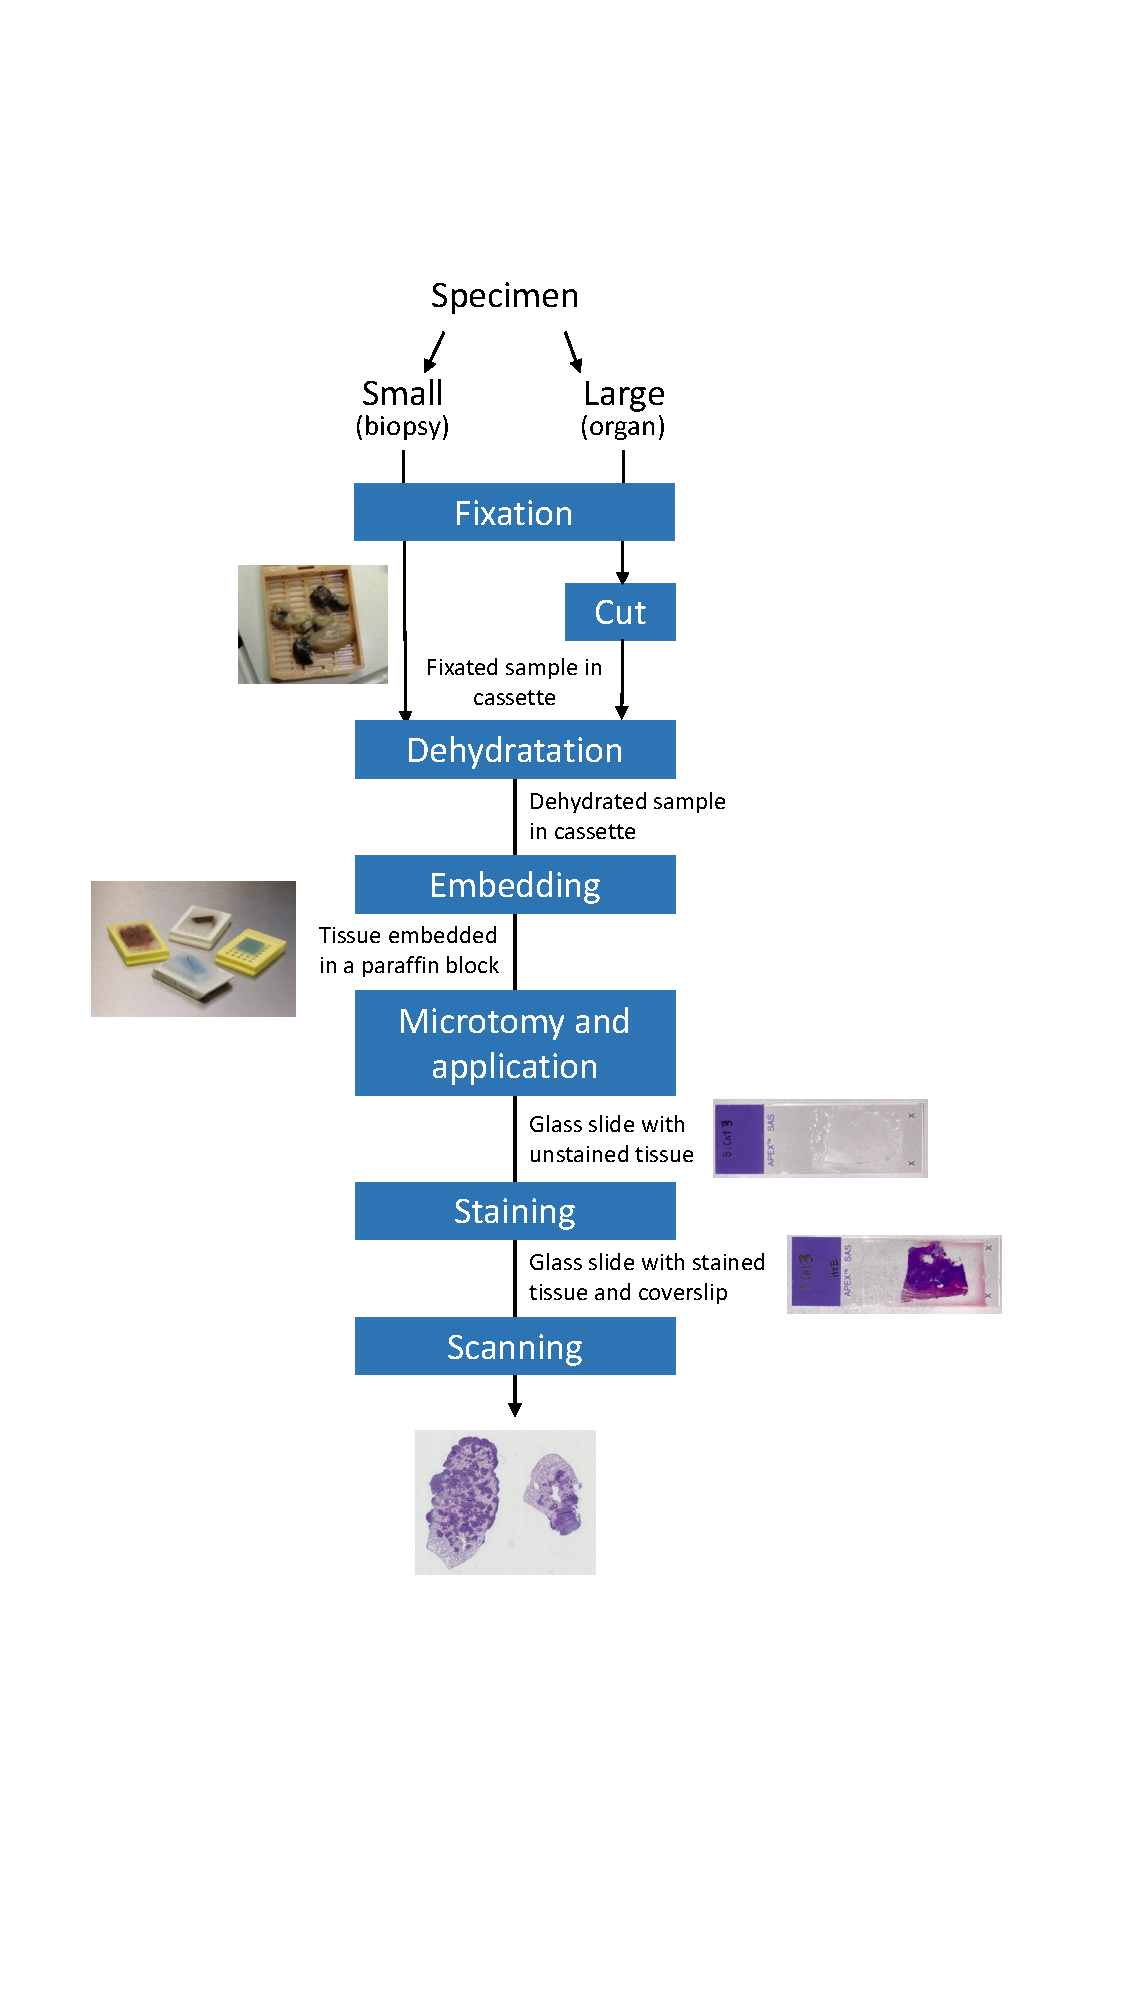
\includegraphics[height=\textheight]{backdp/overallprocess.pdf}
  \caption{Summary of the transformation of a specimen into a \acrlong{wsi}.}
  \label{fig:backdp:overallprocess}
\end{figure}

\subsection{Specimens collection, fixation, cutting and dehydration}

Whether it is for research or diagnosis, the slide preparation process starts with a specimen, a piece of human or animal body for which a question must be answered. The specimen can be as large as a whole organ but can also be as small as a drop of bodily material commonly referred to as a \textit{biopsy}. Before going through the preparation process, a specimen must be fixated. The goal of fixation is to put a stop to the natural decay of the specimen and increase its structural stability \cite{rolls2012process}. This can be achieved, for instance, by immersing the specimen in a formaldehyde bath (\ie the fixative solution) for period of time depending on its size (\ie few hours to a whole day). 

When the specimen has been fixated, it is then placed into a standardized container called a \textit{cassette} (see Figure \ref{fig:backdp:cassette}). If it is too large for the cassette (\eg an organ), one or more volumes of interest are cut from the specimen. Depending on the later examination, the orientation of the cut can be crucial to exhibit relevant tissue structures of the specimen. In the remainder, we will call a \textit{sample} the content of this cassette.

For a proper analysis, the tissue morphology of the sample must be preserved. This is most commonly achieved by infiltrating the tissue with paraffin wax. Infiltration however does not work on a raw fixated tissue because paraffin is hydrophobic. Therefore, one must first perform \textit{dehydration}, that is, replacing water naturally present in the sample with a product miscible with paraffin. This is done by first immersing the sample into a succession of alcoholic solution baths. Although this process achieves dehydration, alcohol does not mix with paraffin neither. Therefore, the sample is then immersed into one or more xylene-based solutions baths, xylene being miscible with both alcohol and paraffin. The sample, infiltrated with xylene, is finally immersed in a paraffin bath under vacuum. The dehydration process takes few hours and is often automated using dedicated machines.

The earliest source of artifacts is the specimen extraction process itself. The specimen can indeed be damaged by the use of certain tools (\eg burned by an electrical scalpel) or treatment at the extraction site. Unlike these, the following artifacts are caused by the early stages of the slide preparation process. Bad fixation can lead to decaying tissue (\ie autolysis, see Figure \ref{fig:backdp:artifacts:autolysis1}) and structural degradation (\eg tissue shrinkage, see Figure \ref{fig:backdp:artifacts:autolysis2}). Improper cutting can also cause tissue damage like tearing and squeezing. Improper dehydration can leave some parts of the sample with remaining water, alcohol or xylene. Tissues can also be exposed to the different solutions for an excessive duration. These processing errors can for instance cause tearing, shrinkage, interference with the staining process (see Section \ref{ssec:backdp:staining}) and affect the structural properties of the tissue (\eg tissue becomes brittle).

\begin{figure}
  \centering
  \begin{subfigure}[t]{0.32\textwidth}
    \centering
    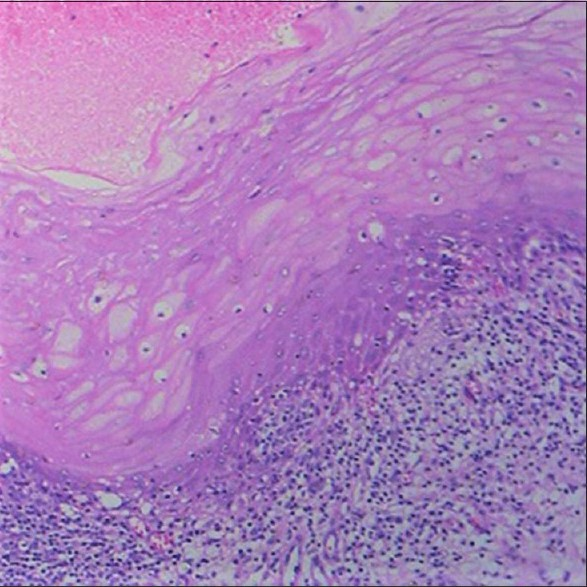
\includegraphics[width=0.98\textwidth]{backdp/JOMFP-22-279a-g007_square.jpg}
    \caption{}
    \label{fig:backdp:artifacts:autolysis1}
  \end{subfigure}%
  \begin{subfigure}[t]{0.32\textwidth}
    \centering
    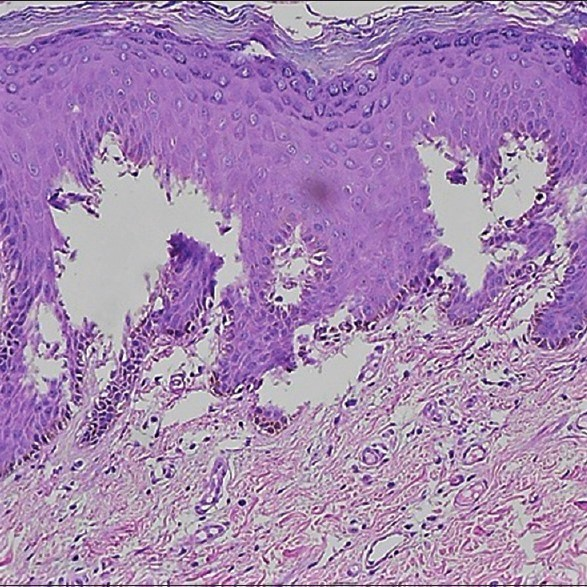
\includegraphics[width=0.98\textwidth]{backdp/JOMFP-22-279a-g008_square.jpg}
    \caption{}
    \label{fig:backdp:artifacts:autolysis2}
  \end{subfigure}%
  \begin{subfigure}[t]{0.32\textwidth}
    \centering
    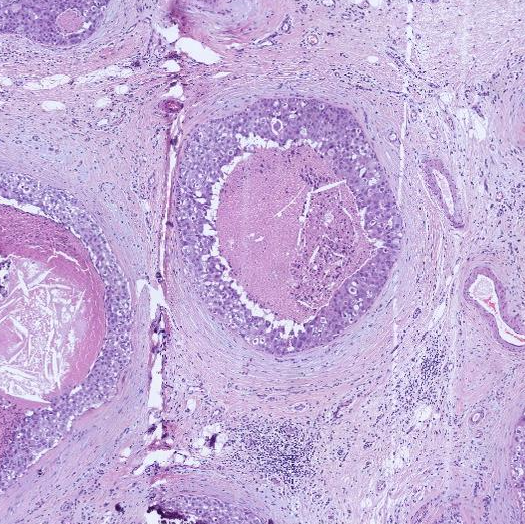
\includegraphics[width=0.98\textwidth]{backdp/artifact_dull_blade.png}
    \caption{}
    \label{fig:backdp:artifacts:microtomy1}
  \end{subfigure}\\

  \begin{subfigure}[t]{0.32\textwidth}
    \centering
    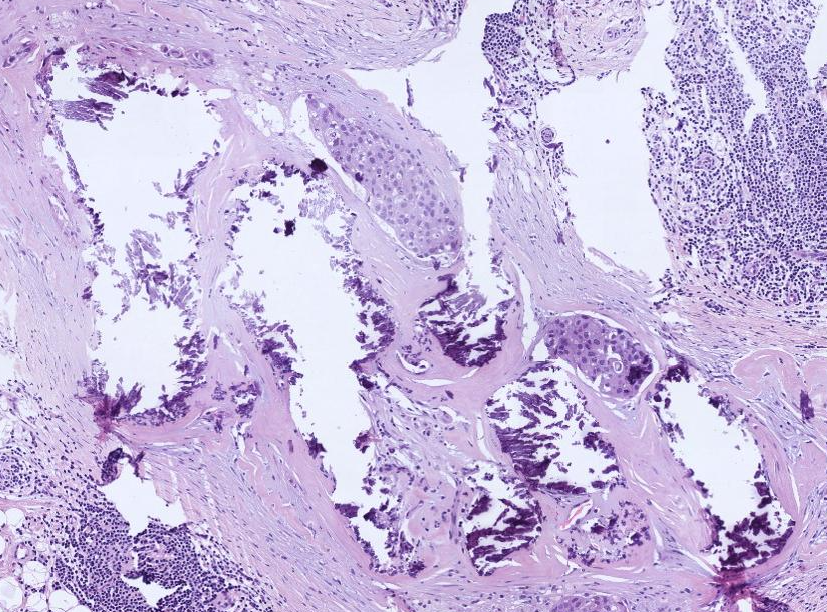
\includegraphics[width=0.98\textwidth]{backdp/calcification.png}
    \caption{}
    \label{fig:backdp:artifacts:microtomy2}
  \end{subfigure}%
  \begin{subfigure}[t]{0.32\textwidth}
    \centering
    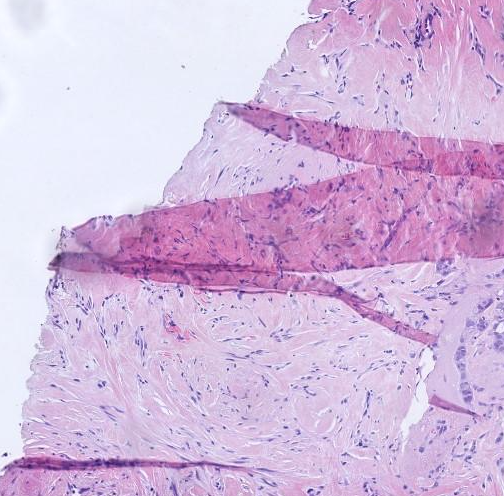
\includegraphics[width=0.98\textwidth]{backdp/folding_artifact.png}
    \caption{}
    \label{fig:backdp:artifacts:folding}
  \end{subfigure}%
  \begin{subfigure}[t]{0.32\textwidth}
    \centering
    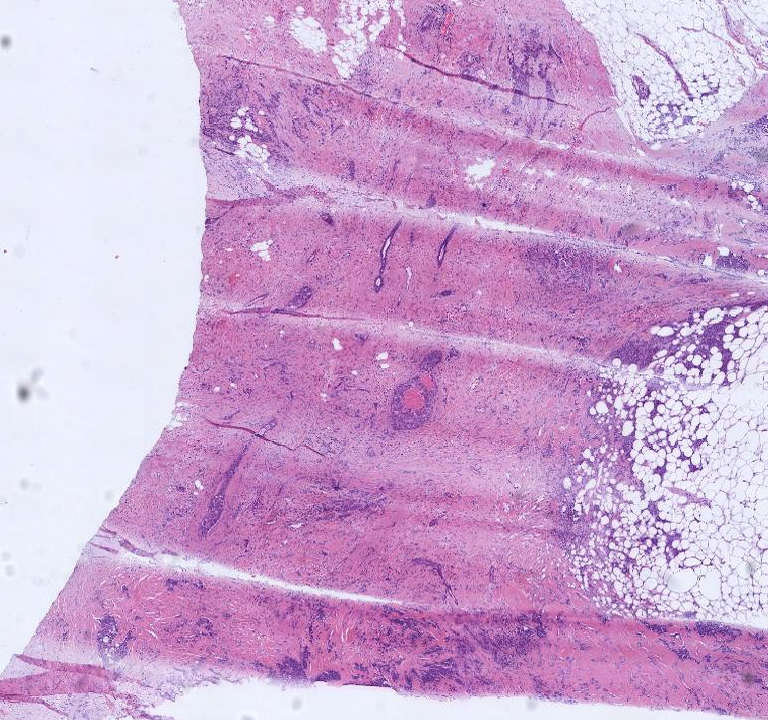
\includegraphics[width=0.98\textwidth]{backdp/staining_artifact.png}
    \caption{}
    \label{fig:backdp:artifacts:staining}
  \end{subfigure}\\

  \begin{subfigure}[t]{0.32\textwidth}
    \centering
    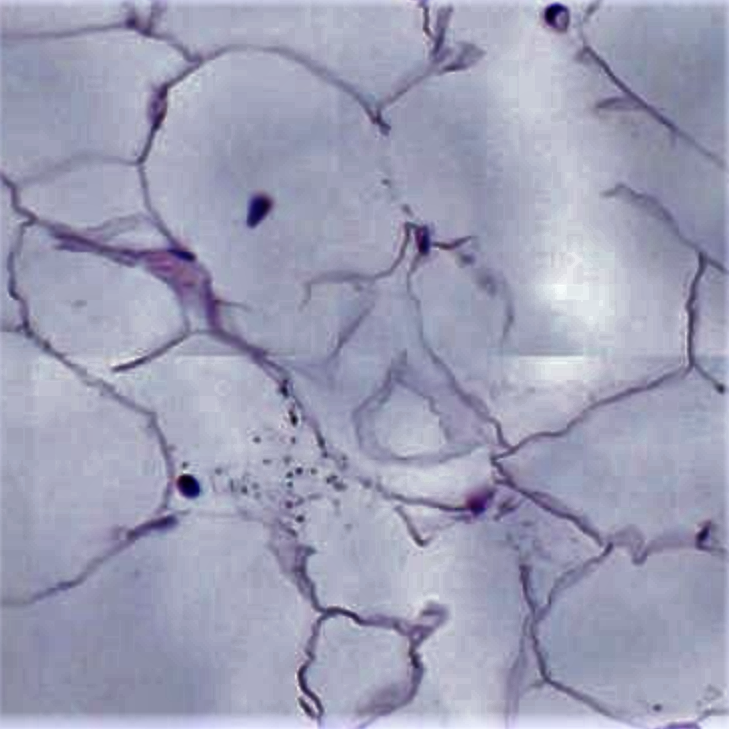
\includegraphics[width=0.98\textwidth]{backdp/artifact_scanner_stitching.png}
    \caption{}
    \label{fig:backdp:artifacts:scanning1}
  \end{subfigure}%
  \begin{subfigure}[t]{0.32\textwidth}
    \centering
    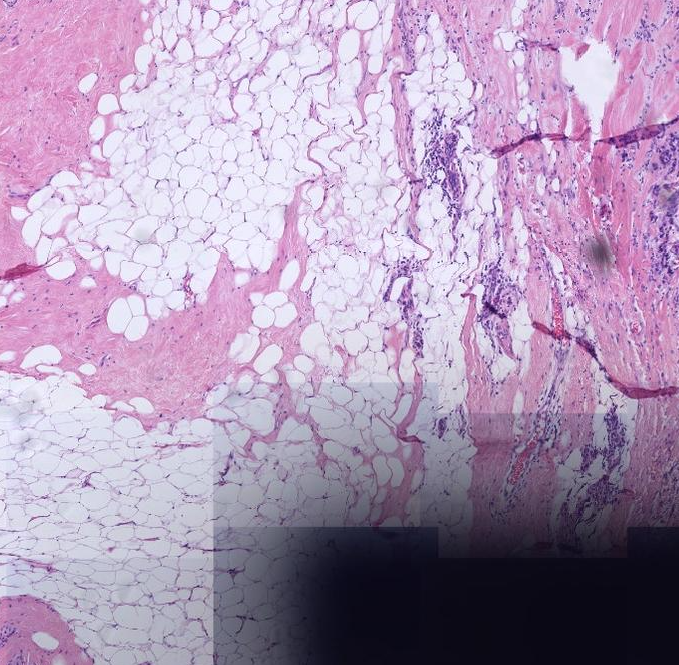
\includegraphics[width=0.98\textwidth]{backdp/scanning_artifact.png}
    \caption{}
    \label{fig:backdp:artifacts:scanning2}
  \end{subfigure}%

  \caption{\textit{Autolysis artifacts}: \ref{fig:backdp:artifacts:autolysis1} (poor cellular differentiation), \ref{fig:backdp:artifacts:autolysis2} (tissue separation). \textit{Microtomy artifacts}: \ref{fig:backdp:artifacts:microtomy1} (nick or blemish in the blade), \ref{fig:backdp:artifacts:microtomy2} (calcification pushed through the tissue by the blade). \textit{Folding artifact}: \ref{fig:backdp:artifacts:folding}. \textit{Staining artifact}: \ref{fig:backdp:artifacts:staining}. \textit{Scanning artifacts}: \ref{fig:backdp:artifacts:scanning1} (stitching issue), \ref{fig:backdp:artifacts:scanning2} (scanner failed to capture part of the tissue) \\ (sources: \ref{fig:backdp:artifacts:autolysis1}, \ref{fig:backdp:artifacts:autolysis2} \cite{taqi2018review}; others from Cytomine).}
  \label{fig:backdp:artifacts:all}
\end{figure}

\begin{figure}
  \centering
  \begin{subfigure}[t]{0.48\textwidth}
    \centering
    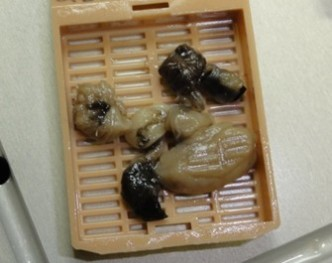
\includegraphics[height=150pt]{backdp/cassette.jpg}
    \caption{Cassette with fixated samples (source: \cite{stidworthy2011getting})}
    \label{fig:backdp:cassette}
  \end{subfigure}\quad
  \begin{subfigure}[t]{0.48\textwidth}
    \centering
    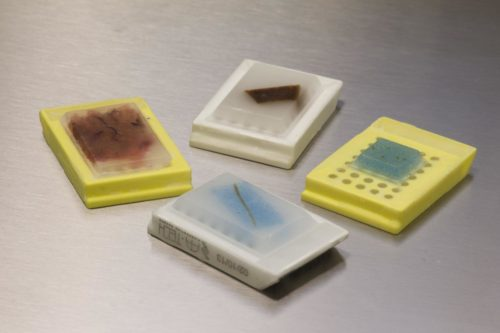
\includegraphics[height=150pt]{backdp/cassette-parrafin.jpg}
    \caption{Cassette with paraffin-embedded samples (source: \cite{img:cassetteparrafin})}
    \label{fig:backdp:cassette-paraffin}
  \end{subfigure}
  \caption{Tissue cassettes.}
\end{figure}

\subsection{Embedding, microtomy and glass-slide application}
\label{ssec:backdp:embedding}

At this point, the sample in the cassette has been infiltrated with paraffin. The next step consists in embedding the infiltrated sample in a block of paraffin to allow easier cutting. The sample is placed in a small container which will serve as a mold for casting the block of paraffin. The cassette is then directly placed on top of the container so that, when the block solidifies, it is attached to the back of the cassette (see Figure \ref{fig:backdp:cassette-paraffin}). When it has indeed solidified, the sample can now be cut into thin slices to be applied on the glass slides. Cutting is performed with a dedicated tool called a \textit{microtome} (see Figure \ref{fig:backdp:microtome}). Operated by a technician, the microtome allows slices to be cut to an extremely small and precise thickness of around 3 or 4 $\mu m$. The slices are then floated onto a water bath which helps mounting them on glass slides. Although there exist equipment that automate the embedding and microtomy steps, to the best of our knowledge, they are not widespread and these steps are still mostly performed by technicians. Even if operated manually, modern microtomes are equipped with automation and ease-of-use features to improve ergonomy and convenience, hopefully improving consistency (\ie slice thickness, \etc.).

\begin{figure}
  \centering
  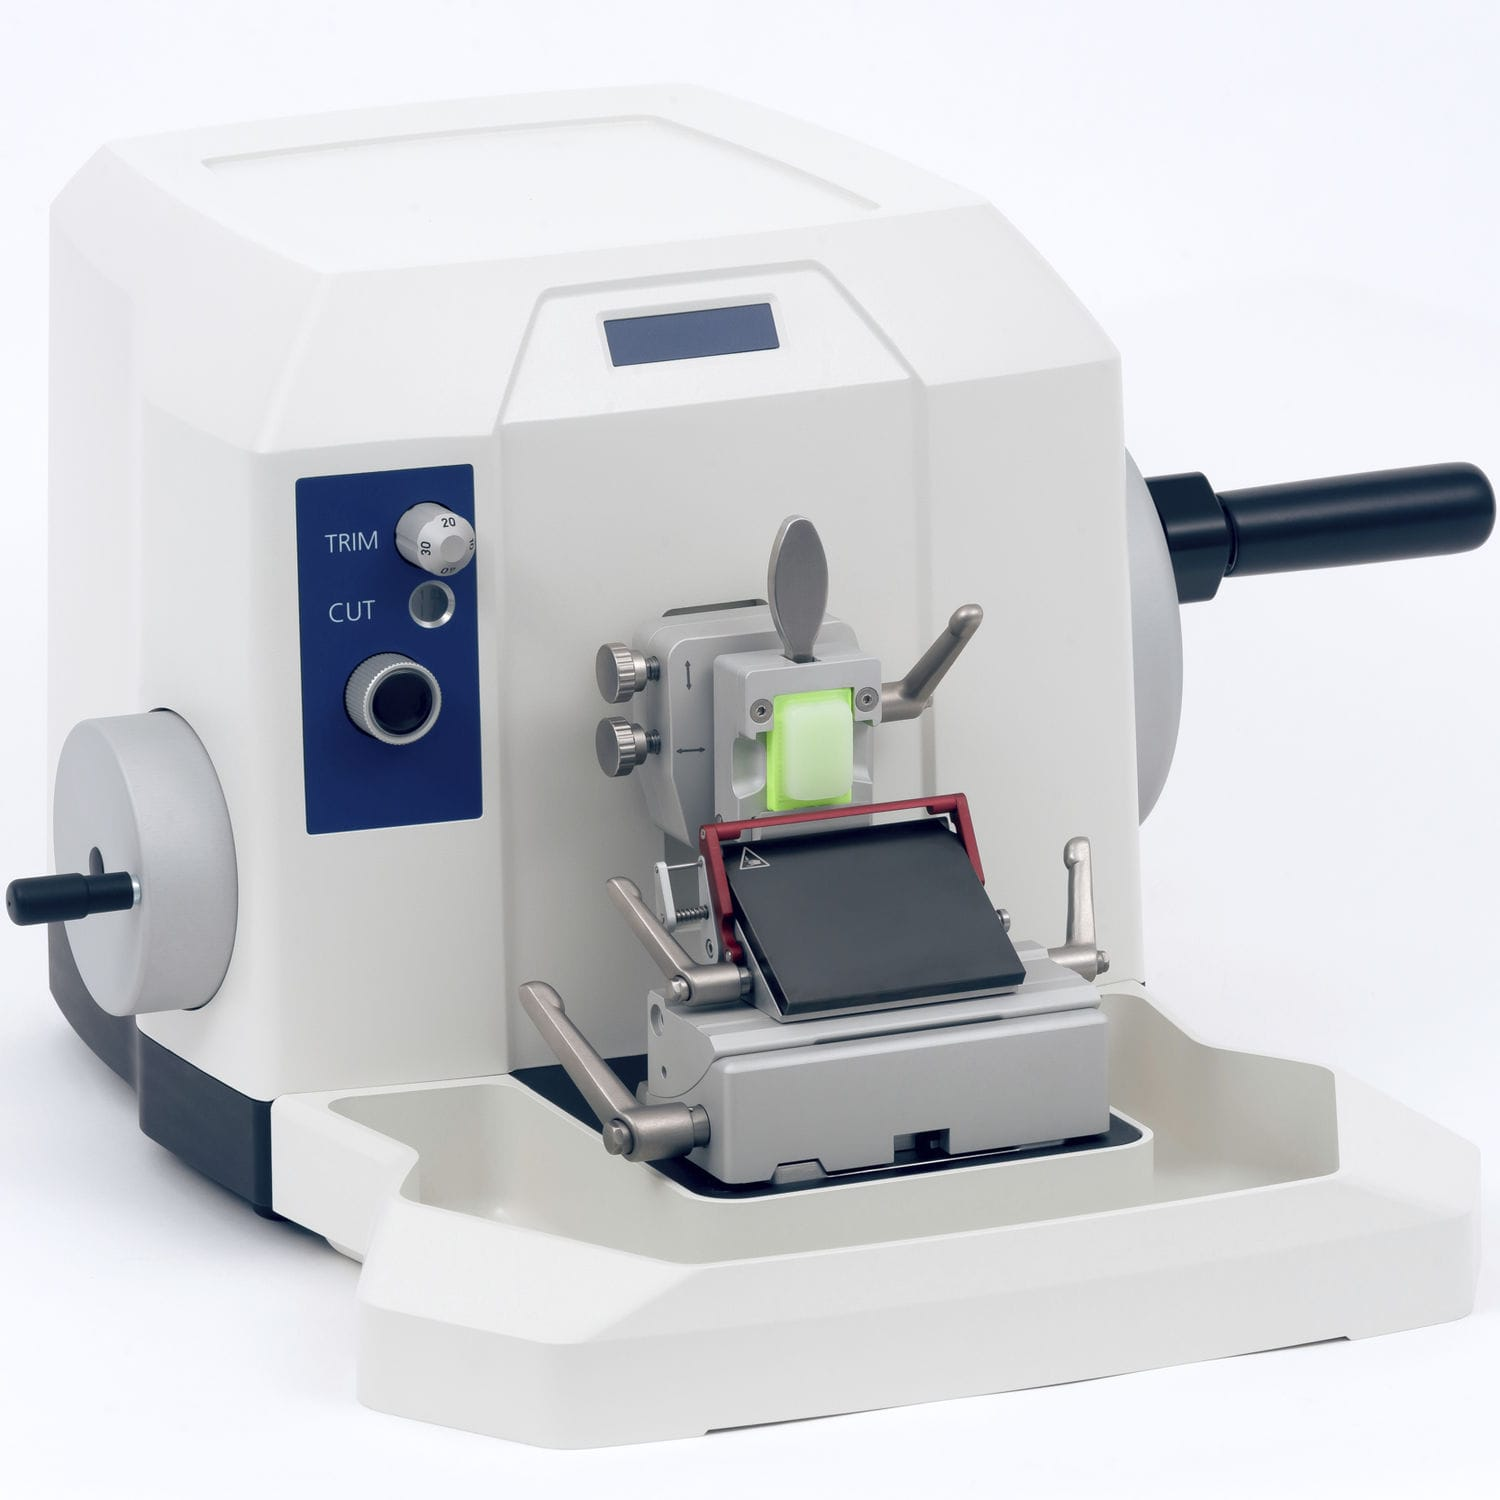
\includegraphics[width=0.5\textwidth]{backdp/microtome.jpg}
  \caption{A microtome.}
  \label{fig:backdp:microtome}
\end{figure}

These steps should be performed carefully not to introduce artifacts. For instance, a warm and soft paraffin block, a dull microtome blade (see Figure \ref{fig:backdp:artifacts:microtomy1}) or a calcification in the tissue can cause compression artifacts (\ie tissue displacement causing material accumulation). A calcification is solid calcium deposit present in the tissue that the blade cannot cut through. This deposit is therefore pushed through the tissue, compressing underlying tissues (see Figure \ref{fig:backdp:artifacts:microtomy2}). Another possible source of artifact is contamination of the water bath with previous samples, hair or dust which can in turn contaminate the floating slices.   

\subsection{Staining}
\label{ssec:backdp:staining}
Mounted tissue slices are almost completely transparent which would prevent any meaningful analysis. They must therefore be stained to highlight structures of interest (see Figure \ref{fig:backdp:stainedvsnonstained}). Similarly as for dehydration, this process consists in immersing the slide into a succession of stainning solutions. The nature of these solutions will depend on the content that should be highlighted for the future analysis. The most common and standard staining in histology is called \acrfirstit{heeo}. Hematoxylin stains nucleic acids in a deep blue-purple color (typically cell nuclei) and eosin non-specifically stains proteins in a pink color (typically extracellular matrix and cytoplasm). The \acrshort{heeo} stain, although most common, is not the only one available. There exist many other staining techniques such as \acrfirstit{ihc} which exploits the binding nature of some antibodies with specific proteins. Markers can then be used to highlight the antibodies, hence the proteins of interest they have bound with. Because the \acrshort{ihc} staining can be very selective, a counterstain (\eg hematoxylin) is often applied to highlight the rest of the tissue. Counterstain is particularly important when different slices of a tissue stained with different techniques must be compared together because it helps matching the slices spatially. An example of a tissue stained with \acrshort{heeo} and \acrshort{ihc} is given in Figure \ref{fig:backdp:heeo-ihc}. When the sample has been stained and cleaned from remaining excess of staining solutions, one must apply a cover slip on the sample in order to ensure that sample lies in one single plane as the focal plane of microscopes and scanners is usually quite narrow. The cover slip also protects the sample from external contamination and degradation. 

\begin{figure}
  \centering
  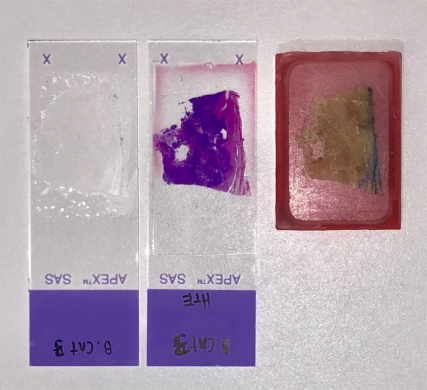
\includegraphics[width=0.6\textwidth]{backdp/staindvsnonstained.png}
  \caption{\textit{Left:} an unstained tissue section mounted on a glass slide. \textit{Middle:} \acrshort{heeo}-stained section coming from the same tissue. \textit{Right:} the source tissue embedded in a paraffin block \\ (source: \cite{abbasi2019all}).}
  \label{fig:backdp:stainedvsnonstained}
\end{figure}

The choice of a staining and its clean application are crucial for an efficient analysis. The staining baths can become contaminated with samples, by-products resulting from chemical reactions (\eg precipitation or crystallization of chemical components resulting in the presence of pigments in the sample) or external objects (\eg hair, dust). The baths tend to degrade over time as moving slides from one bath to another transfer some staining solutions as well. The degradation of the staining solutions can cause variation in staining intensities between earlier and later samples. The bath duration is important for proper staining and bathing samples for less or more time than recommended can respectively cause under- or over-staining (see Figure \ref{fig:backdp:artifacts:staining}). Moreover, insufficient cleaning after staining can leave spots of stain on the slide. Improper application of the cover slip can for instance cause the presence of air bubbles. 

Nowadays, the staining process can be automated with automated slide stainers. These systems move the slide automatically from a bath to the next ensuring stable dipping durations for each stain.

\begin{figure}
  \centering
  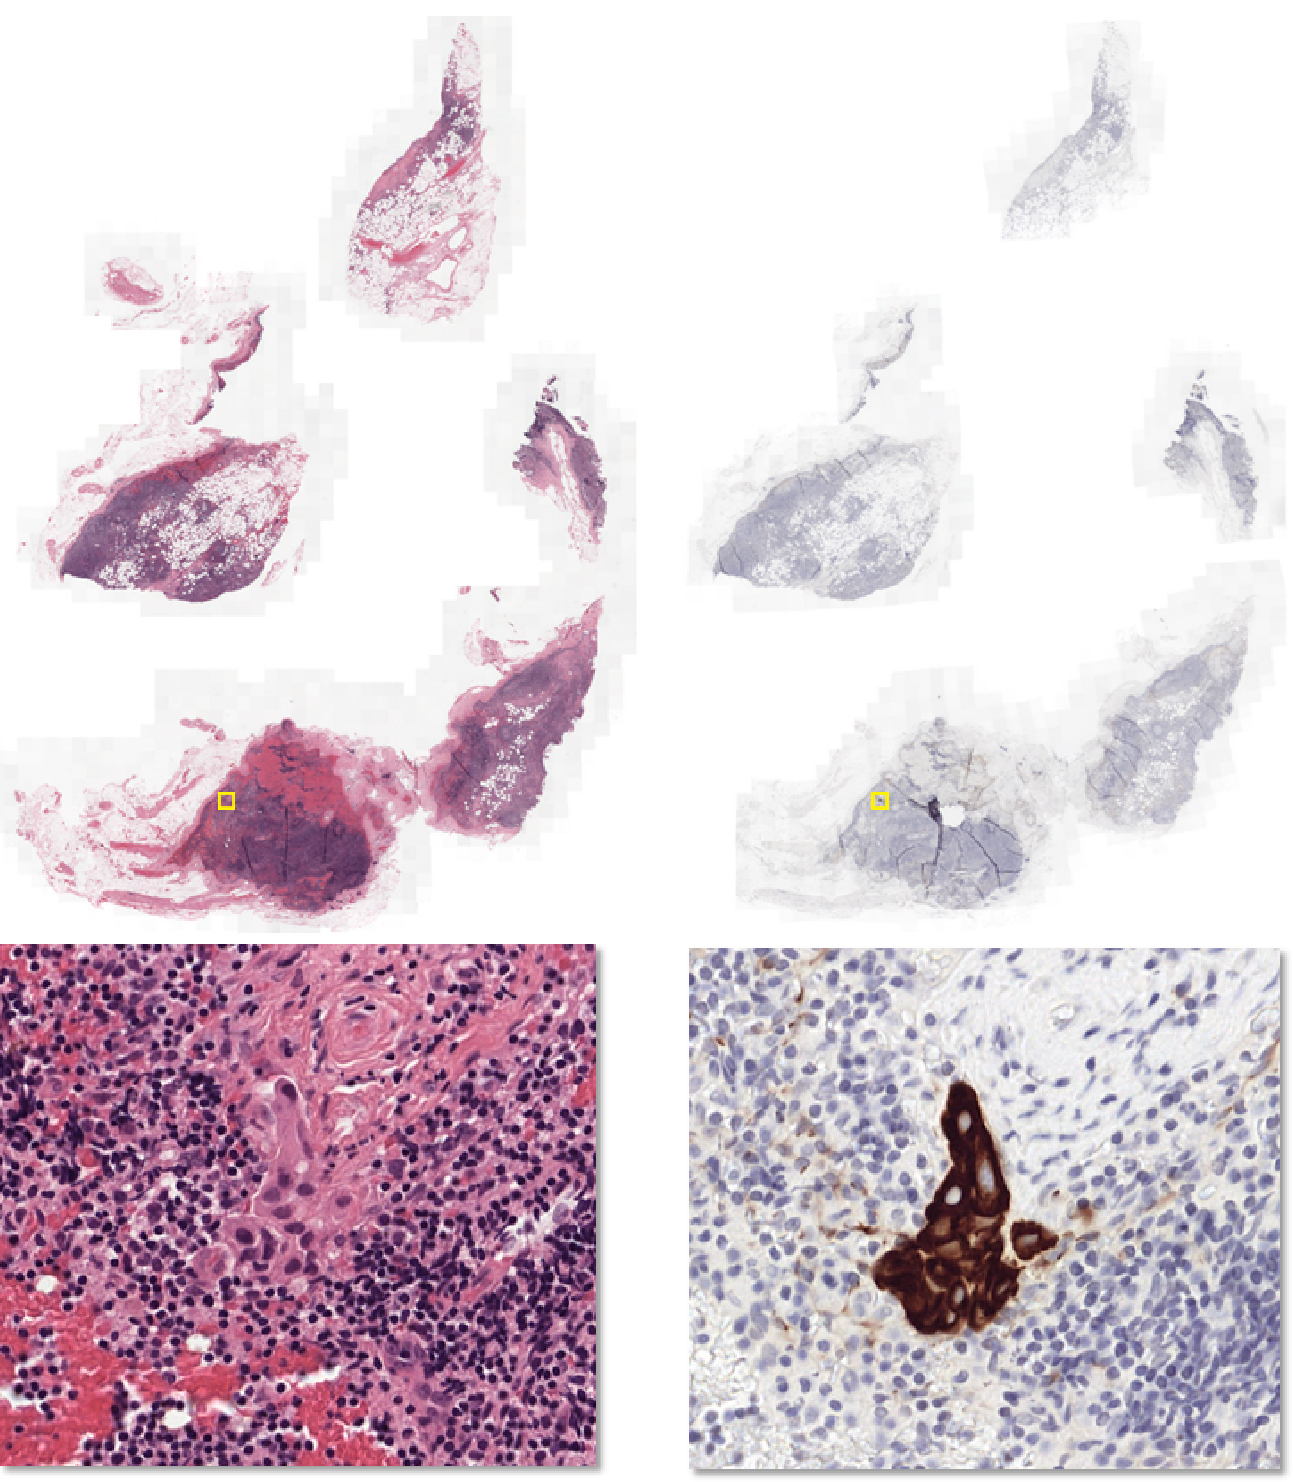
\includegraphics[width=0.5\textwidth]{backdp/heeo-ihc.jpg}
  \caption{Two slices of the same tissue stained with \acrshort{heeo} (left) and \acrshort{ihc} (right) (source: \cite{litjens2018camelyon}).}
  \label{fig:backdp:heeo-ihc}
\end{figure}

\subsection{Scanning}
\label{ssec:backdp:scanning}

A glass slide coming out of the staining process described in Section \ref{ssec:backdp:staining} is ready to be analyzed with an optical microscope but can also be digitized by a slide scanner into a \acrshort{wsi}. In this section, we will briefly describe few key elements related to slide scanning. A more thorough technical presentation and discussion of scanning technologies can be found in \cite{patel2021contemporary}. 

Scanners are equipped with high-precision lenses and sensors allowing them to generate very high-resolution images required for a proper analysis. Magnification and resolution are two popular metrics used to describe the visual quality of the resulting image. Magnification advertised by scanner vendors refers to the maximum size of the objects in the scanned image with typical values being $\times$20 or $\times$40 (\ie objects appear 20 or 40 times larger than they actually are). Resolution determines the extent to which smaller objects can be resolved. Resolution is reported for a given magnification level and often lies around 0.25 $\mu$m/pixel at $\times$40 for modern scanners but higher magnification and resolution are possible. These magnifications are standard and, coupled with an adequate resolution, are usually sufficient for routine analysis of \acrshort{heeo} or \acrshort{ihc} slides \cite{zarella2019practical}.

\begin{figure}
  \centering
  \begin{subfigure}[t]{0.48\textwidth}
    \centering
    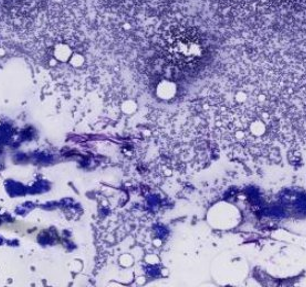
\includegraphics[height=190pt]{backdp/magres_x1.25_cell.png}
    \caption{$\times$1.25, 7.24 $\mu$m/pixel}
  \end{subfigure}
  \begin{subfigure}[t]{0.47\textwidth}
    \centering
    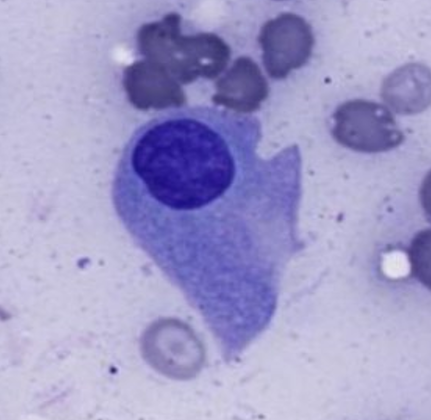
\includegraphics[height=190pt]{backdp/magres_x40_cell.png}
    \caption{$\times$40, 0.226 $\mu$m/pixel}
  \end{subfigure}
  \caption{Two images (approximately 200 $\times$ 200) extracted from the same WSI at different magnification and resolution (reported in subcaptions). They are both centered on the same cell.}
\end{figure}

Given the need for high magnification and resolution, it is not possible to capture the whole slide in a single shot with currently available sensors. Therefore, scanners typically capture a sample step by step either tile by tile or in an in-line fashion and then assemble together the different parts using a stitching algorithm. Obviously, as a slide is scanned in several shots, the scanner must ensure that focus is correct for all the shots in order to avoid blur. Common focus strategies are for instance re-focusing every tile, or every $n^{\text{th}}$ tile. When it comes to the focus strategy, there is usually a trade-off between scanning time and focus precision: focusing every tile allows for ideal focus but takes time, whereas focusing every $n^{\text{th}}$ is faster but incurs a risk of incorrect focus and blur between the re-focusing steps. Modern scanners implement efficient strategies to reduce the scanning time per slide which nowadays ranges from 30 seconds to several minutes (at $\times$20 or $\times$40 magnification). These strategies include improved focus strategies and automatic tissue detection allowing to skip the empty parts of the slide during scanning. Most scanners also allow to load batches of few hundreds of slides at once therefore reducing the time spent by the operator interacting with the machine.

For histology, it is usually sufficient for scanners to scan one focal plane of the slide (\ie that of the tissue slice). For cytology, however, it is not always enough. Indeed, the slide preparation process for a cytology sample differs and the material is not always aligned within a single focal plane. With an optical microscope, it is possible to navigate continuously over the focal planes by adjusting the lenses positions. When it comes to scanning such samples, one has to resort to a technique called "\textit{z-stacking}". It consists in capturing the material at different depths along the $z$-axis. This process can be significantly longer than single focal plane scanning, as it multiplies this time by the number of slices of the stack. The result is a finite number of images which can be viewed in different ways (\eg one by one, grid view, as a video sequence, \etc.) but does not offer the simplicity or continuous exploration provided by optical microscope for this task. 

Scanning can also introduce artifacts including stitching problems (\ie misalignment between scanned tiles or lines, see Figure \ref{fig:backdp:artifacts:scanning1}), blur due to incorrect focus, tissue detection failure causing parts of the slide to be missing from the \acrshort{wsi} (see Figure \ref{fig:backdp:artifacts:scanning2}). The scanner should obviously remain as clean as possible to avoid external components to pollute the image (\eg dust, glass shards, hair, \etc.). 

\subsection{File formats and compression}
\label{ssec:backdp:storingviewing}

For each glass slide, a scanner generates one or more files to store the image data but also any metadata related to the case (information or identifiers of laboratory, patient, specimen, staining, \etc.). How the data is organized in such a file is specified by a \textit{file format} of which there exist many. Some file formats are closed and proprietary (\eg scanner- or vendor-specific file formats) but others have open specifications (\eg DICOM, OME-TIFF). The most involved formats usually combine a descriptive part to store case-related metadata using, for instance, the XML language (\eg in OME-TIFF) and a subfile format for the image itself (\eg TIFF). 

Regarding the internal structure of the latter, the image is usually splitted into a set of tiles (\eg 1024 $\times$ 1024) rather than being stored as a single image array. The file contains metadata to provide efficient access to these tiles. This organization makes sense because, in practice, one rarely has to load the whole image in memory at full resolution at once which, given the size of a raw image (\eg Figure \ref{fig:backdp:pyramidalimage}), would be impossible on most computers anyway. It is however a common use case for a practitioner to look at an entire slide (or a large region of interest) at a lower magnification and resolution. Downsizing, downsampling and aggregating tiles to obtain a low resolution view of a slide (or a region of interest) is an expensive operation and cannot realistically be performed on-the-fly without significantly increasing loading times. Therefore, a typical image files also stores versions of the image at different zoom levels. The $i^{\text{th}}$ zoom level ($i \in \mathbb{N}_0$) is a version of the image which has been downsized by a factor $2^i$ (or $3^i$, $4^i$ depending on the image format). The number of zoom levels varies depending on the size of the image at full resolution and is such that the image at the lowest zoom level (\ie largest $i$) has a reasonably low size (\eg when it fits in a single tile). Similarly as for zoom level 0, other zoom levels are stored as set of tiles. Such a file is called \textit{pyramidal} because of this structure (see Figure \ref{fig:backdp:pyramidalimage}).

\begin{figure}
  \centering
  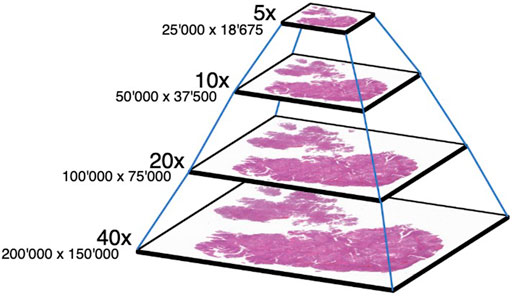
\includegraphics[width=0.75\textwidth]{backdp/pyramidalimage.jpg}
  \caption{Pyramidal view of a whole-slide image (source: \cite{marini2022multi_scale_tools}).}
  \label{fig:backdp:pyramidalimage}
\end{figure}

A whole-slide image file is not a lightweight one. For example, a raw $10^5 \times 10^5$ RGB image (3 bytes per pixels) contains 30 gigabytes of information. This is massive and not scalable if one has to consider the multitude of slides to be scanned and stored by an hospital for instance. Therefore, compression algorithms are very frequently used to reduce the size of image files. Popular choices are JPEG (lossy compression) and JPEG2000 (lossless compression). Compared to its lossless counterpart, lossy compression allows for better compression rate and disk usage reduction. However, the loss of information results in visual alterations that become more and more severe as the compression rate increases. Therefore, lossy compression should be used carefully to avoid destroying image features relevant to the analysis. 

\subsection{Visualization and hardware considerations}
\label{ssec:backdp:visualization}

An image file is not worth much if it cannot be viewed. Nowadays, there exist many open or proprietary software and tools for visualizing \acrshort{wsi}. Some are desktop applications designed to run on personal computers and workstations (\eg QuPath \cite{bankhead2017qupath}, ASAP \cite{cpg2022asap}) and some others are directly provided by scanner vendors to run on dedicated hardware alongside the scanner. Some others are web-based (\eg Cytomine \cite{maree2016collaborative}, OMERO \cite{allan2012omero}) for which the viewer can be accessed through a web browser and content is served over the HTTP protocol. The most popular tools are not limited to a viewer but usually include many more features. For instance, Cytomine includes image annotation tools, integration of computer vision and \acrlong{ml} algorithms, authentication, project-based content organization, an \acrshort{api} to interact with data programmatically, \etc.

Whereas it is included by-design in web-based tools, remote slide viewing is also possible with some desktop applications. This feature is particularly important in a laboratory environment. Without it, the system would need to download an entire \acrshort{wsi} file before being able to display. This would add a significant latency in the slide reviewing process. Remote slide viewing allows for a seamless and more efficient interaction between the practitioner and the viewing system.

Beyond software, hardware considerations are important for efficient viewing, especially when implemented at the scale of a laboratory or pathology service \cite{temprana2022digipatics}. Personnal workstations should be equipped with a quality screen able to render image without loss of quality (color and resolution) \cite{rojo2015analysis}. They also must be equipped with adequate computing resources (memory and \acrshort{cpu}/\acrshort{gpu}) in particular if analysis algorithms are supposed to be executed on them. The network should be robust enough to support the exchange of information (\ie download and upload of large files and data). Servers should have enough disk space to store the digitized slides and data and implement mechanisms in order to minimize the risk of data corruption or loss. 

\subsection{Discussion}

As presented in the previous sections, the preparation process has a significant impact on the final quality of a slide. Every step in the process introduces variability and has a chance of creating artifacts that can be both harmful to the analysis. Fortunately, automation reduces significantly the variability and makes the risk of artifacts acceptably low, although not absent. The dehydration, paraffin embedding and staining steps can all be automated with dedicated machines nowadays but microtomy remains mostly manual due to the high-precision requirements of the process. For scanned slide, there exist automated quality control tools such as HistoQC \cite{janowczyk2019histoqc} or PathProfiler \cite{haghighat2021pathprofiler} to verify that a \acrshort{wsi} has a sufficient quality to be considered for analysis. 

The preparation process also impacts significantly the diagnosis time as overall, from fixation to scanning, it can take from 12 to 24 hours (sometimes more) to obtain a slide depending on the nature and state of the original specimen. There exist faster processes such as cryosectioning (\ie the sample is frozen then sectioned) for intraoperative consultation during which a surgeon requests an analysis to decide how to proceed with a surgical operation. Such process can provide an answer within the hour but the resulting slides are usually of lesser quality than traditionally prepared histological slides.

\section{Whole-slide analysis}
\label{sec:backdp:typicalanalysistasks}

When a slide has finally been prepared, a pathologist, a biologist or a technician can take over and start the analysis, whether on a computer screen or through the lenses of an optical microscope. There exist many active research domains which rely on slide analysis. Similarly, there exist many pathologies that can be discovered from the same source. For the sake of simplicity, the remainder of the section will focus on oncology and cancer diagnosis. In this field, one of the most frequent conditions that has to be evaluated is malignancy of tumors. The indicators of malignancy can vary greatly from a disease to another and even from one type of cancer to another. The approach of the slide by the pathologist and the analysis can therefore vary accordingly.

Two important tools for diagnosis and prognosis of cancer are grading and staging systems. A grading system is a set of mostly objective criteria for evaluating how abnormal cancer cells and tissues are compared to their healthy counterparts. Similarly, a staging system defines a set of criteria for quantifying the dimensions of the primary tumor and determining how far the cancer has spread in the patient's body. These criteria can be quantitative (\eg cell counts, tumor area dimensions) or qualitative (\eg cell or tissue morphology, presence of metastases) and consider macroscopic or microscopic elements. Beyond grading and staging, slide analysis can also provide direct information for establishing a proper treatment. For instance, localizing a malignant tumor in its support tissue can be important for guiding a future surgical operation. 

All the types of tasks involved in slide analysis are not equal. They have varying degrees of complexity and tediousness. Some tasks are rather simple but take a significant amount of time (\eg counting mitosis, see Section \ref{ssec:backdp:analysis_mitotic_count}), others require strong focus for an extended period of time which increases the risk of error (\eg thyroid nodule malignancy, see Section \ref{ssec:backdp:analysis_thyroid}). Moreover, some diagnoses require to screen more than just one slide, in which case the volume of information to review can be significant. 

When a task has to be performed frequently and is tedious, error-prone or involves reviewing a large amount of data, there is a great potential for \acrlong{cpath} methods to improve analysis quality and speed. These methods can either provide quantitative or qualitative information that directly contributes to the diagnosis or simply assists the practitioner during the reviewing process. % (\eg image registration, see Section \ref{ssec:backdp:analysis_registration}). 

Beyond automating existing tasks, \acrlong{cpath} could also give rise to new approaches and standards for diagnosis. For instance, computational methods could be used to extract new descriptive features such as exhaustive statistics about cell types and structure in a sample or new cell morphology descriptors. This information could be used alongside non-imaging data and correlated to patient outcome \cite{abels2019computational}. 

In the longer term, new computational methods coupled with new imaging techniques could make obsolete the slide preparation process as it is performed now as well as the current diagnosis systems based on histology and cytology. Indeed, in the future, entire specimen could be scanned directly to produce 3D volumes with slide-free microscopy techniques \cite{np2017histopathology, liu2021slide}. These image volumes could be analyzed directly by computational methods to provide fast and hopefully reliable indicators for pathologists to diagnose cases in a shorter time frame than ever before. However, it will take a significant amount of time before such technology is sufficiently developed, validated and becomes reliable enough to be used in clinical practice on a daily basis. 

In the following sections, we provide some examples on diagnosis tasks that would greatly benefit from automation with computational methods. For each of them, we also provide examples of contributions of the \acrlong{cpath} community to the automation of these tasks. The datasets presented in these sections were used in the contributions of the thesis. 

\subsection{Mitotic count}
\label{ssec:backdp:analysis_mitotic_count}

Mitosis is one of the phases of the cell cycle during which the chromosomes (replicated in a previous phase) are separated into two new nuclei. Tumor often exhibit a larger mitosis rate compared to healthy tissues. Many grading systems therefore use a measure of the mitosis rate as an indicator of cancer severity. For instance, the Bloom-Richardson system \cite{roychowdhury2022bloomrichardson} for histologic grading of breast cancer includes mitotic count as one of its three indicators. In particular, mitosis must be counted in 10 fields of view. The final grade is determined based on a point system. Each indicator provides 1 (least severe) to 3 (most severe) point(s) which are added together (3-5 pts = grade I, 6-7 pts = grade II and 8-9 pts = grade III). For the mitosis indicator, 1 point is given if the mitotic count is 5 or less, 2 points if it is between 6 and 10 and 3 points if it is 11 or more\footnote{The recommended numbers might change based on the microscope used for the analysis.}. 

Counting mitosis is cumbersome. It is no surprise that \acrlong{cpath} methods have been investigated to automate the task. For example, in 2014 was organized the MITOS-ATYPIA-14 challenge \cite{roux2014mitos} where participants had to come up with the best \acrlong{ml} model to count the number of mitosis in different fields of view (see Figure \ref{fig:backdp:mitos_atypia}). In addition to the mitotic count, they had to predict a global nuclear atypia score for each field of view, nuclear atypia being another indicator of the Bloom-Richardson system. 

\begin{figure}
  \centering
  \begin{subfigure}[t]{0.48\textwidth}
    \centering
    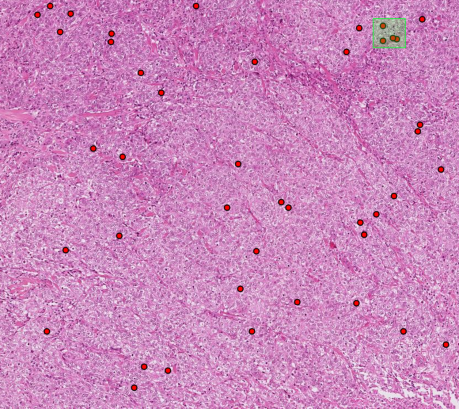
\includegraphics[height=190pt]{backdp/mitosis_zoomout.png}
  \end{subfigure}
  \begin{subfigure}[t]{0.48\textwidth}
    \centering
    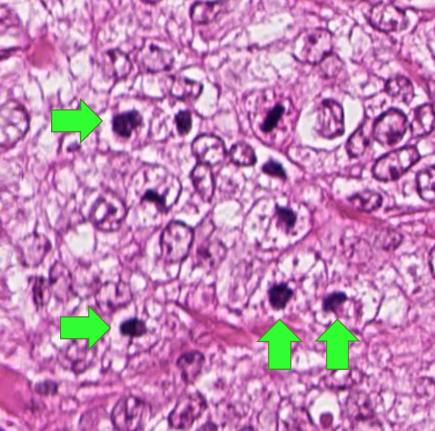
\includegraphics[height=190pt]{backdp/mitosis_zoomin.png}
  \end{subfigure}
  \caption{\textit{Left:} a training image provided for the MITOS-ATYPIA-14 challenge viewed from the Cytomine viewer. Red dots are mitosis present in this image. \textit{Right:} A close up view of four mitosis (in the green square from the left image).}
  \label{fig:backdp:mitos_atypia}
\end{figure}

\subsection{Breast cancer staging and sentinel lymph nodes}
\label{ssec:backdp:analysis_camelyon}

Axillary lymph nodes are structures of the immune system located near the armpit. They drain a large proportion of the lymph coming out of the breast. They contain lymphocytes and constitute a barrier that eliminates bacteria, viruses and other foreign particules (including metastases) from the lymph. Because they are the first recipient of metastases originating from breast tumors, these lymph nodes are an important element to consider when staging breast cancer. In particular, in the context of $TNM$, a standard internationally accepted cancer staging system, the $pN$-stage \cite{reisenbichler2022tmnstagingbreast} quantifies cancer spread through the presence of metastases in regional lymph nodes. Its histological evaluation requires to screen one section of up to 10 axillary lymph nodes and several sections of the ``sentinel'' lymph node which is the most likely to contain metastases \cite{weaver2010pathology}. Sometimes, additional slides counter-stained with \acrshort{ihc} must be analyzed to confirm the diagnosis. The staging system requires to evaluate the number of nodes contaminated with metastases and the dimensions of these metastases (\ie their size and the number of cells they contain).

Evaluation of the $pN$-stage has many characteristics that qualifies it to be a good candidate for automation: it is time-consuming, tedious and error-prone. The computational pathology community has therefore considered this problem notably through the Camelyon16 and Camelyon17 challenges \cite{litjens2018camelyon}. For the first iteration of the challenge, the participants had to predict a slide-level $pN$-stage. For the second iteration, the organizers moved to a patient-level prediction. The participants were provided with 899 training and 500 testing \acrshort{wsi}s which were collected in 5 different hospitals and medical centers from the Netherlands. All training slides were also coming with a slide level $pN$-stage label. Moreover, 209 of those \acrshort{wsi}s contained detailed hand-drawn contours for all metastases (see Figure \ref{fig:backdp:camelyon_sample}). The top-performing solutions typically used a combination of techniques and algorithms including traditional computer vision pre- and post-processing methods, \acrlong{dl} to segment the metastases and rule-based or random forests methods to predict the final stage. 

This challenge was a success as many teams participated despite the complexity of handling such a massive dataset (3 terabytes of slide data). The top-performing algorithms were quite successful at predicting the $pN$-stage. However, as stated by the organizers, the task was not adequatly solved and there was room for improvement \cite{bandi2018detection} as a combination of the best algorithms still misclassified the $pN$-stage for 23 patients out of 100. 

\begin{figure}
  \centering
  \begin{subfigure}[t]{\textwidth}
    \centering
    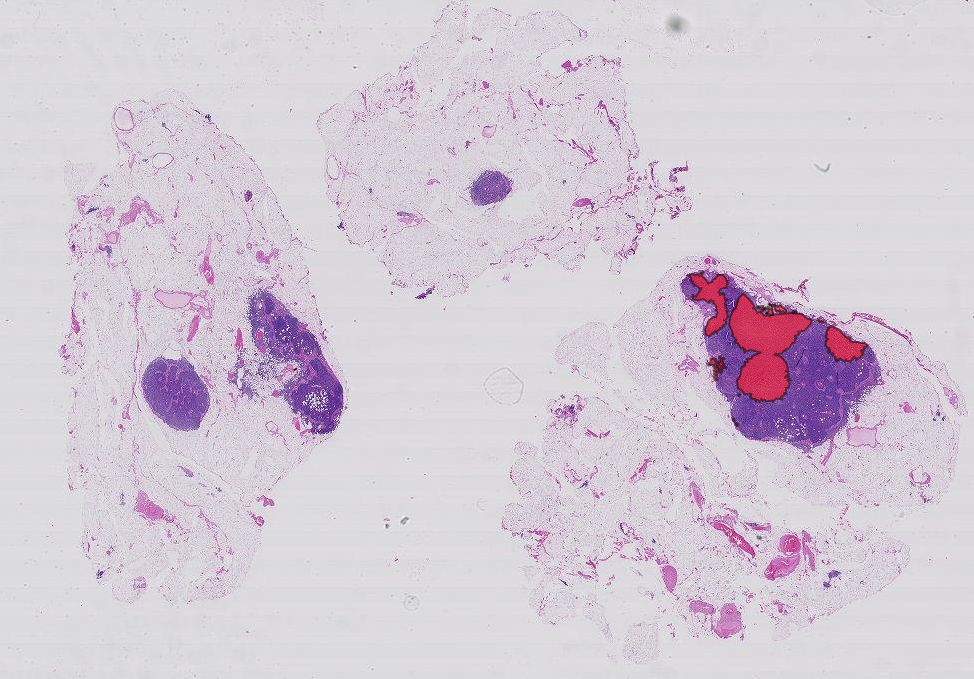
\includegraphics[width=\textwidth]{backdp/camelyon_lymphnode.png} 
  \end{subfigure}\\
  \vspace{1cm}
  \begin{subfigure}[t]{0.48\textwidth}
    \centering
    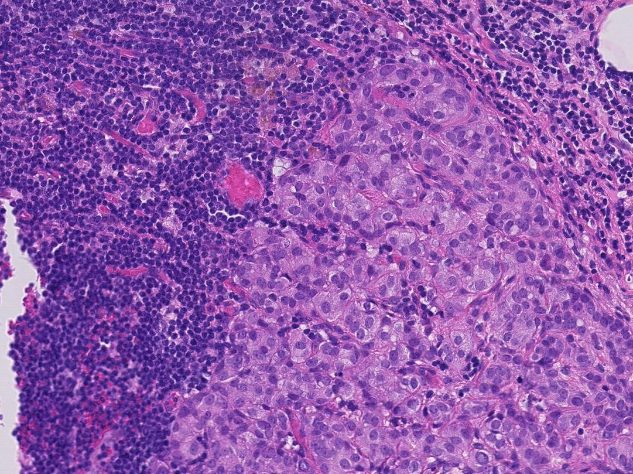
\includegraphics[height=150pt]{backdp/camelyon_metastase_noannot.png}
  \end{subfigure}
  \begin{subfigure}[t]{0.48\textwidth}
    \centering
    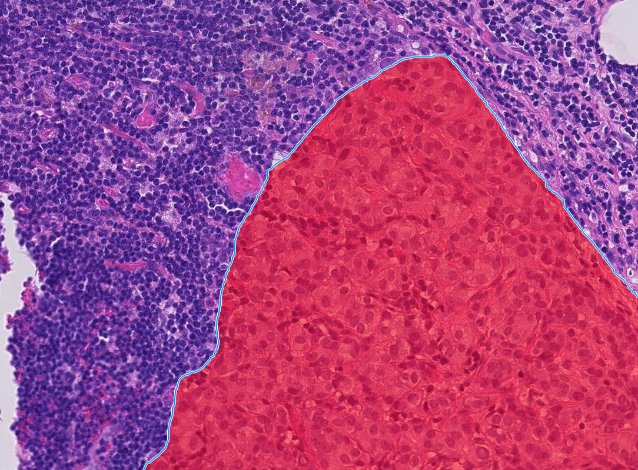
\includegraphics[height=150pt]{backdp/camelyon_metastase_withannot.png}
  \end{subfigure}
  \caption{A \acrshort{wsi} from the Camelyon16 challenge training set viewed from the Cytomine viewer. \textit{Top:} the whole-slide image with metastases highlighted in red. \textit{Bottom:} A close-up view of a metastase with (\textit{right}) and without (\textit{left}) annotation mask.}
  \label{fig:backdp:camelyon_sample}
\end{figure}

\subsection{Thyroid nodule malignancy}
\label{ssec:backdp:analysis_thyroid}

A thyroid nodule is a small lump that can form within the thyroid gland. Most nodules are benign but up to $5\%$ of them are malignant \cite{yeung2008management}. Malignancy diagnosis is based on a wide variety of information including patient history (past exposure to radiation, family history of thyroid cancer, \etc.) and different technical examinations (\eg echography or radiography). A crucial step in the process is the \acrfirstit{fnab} during which cell material is extracted from the nodule. The resulting cytology sample is smeared on a glass slide (this slide preparation process is different from the one described in Section \ref{sec:backdp:wsi}), stained and examined under a microscope. Cytology analysis is an integral part of the Bethesda diagnosis system \cite{bychkov2022bethesda} which grades a nodule into six categories going from nondiagnostic (TBS I) and benign (TBS II) to malignant (TBS VI). One of the elements that define the TBS category is the presence of cells with intranuclear inclusions (see Figure \ref{fig:backdp:thyroid_inclusion}) which are highly suggestive of malignancy \cite{arena2014intranuclear}. Relatively to the size of a slide, these cells are tiny and the problem of finding them comes down to searching a needle in a haystack (see Figure \ref{fig:backdp:thyroid_needle_haystack}). However, these cells are not the only indicators of thyroid cancer and considering this is only a part of what must be investigated in a thyroid nodule smear, it would greatly benefit from the use of computational methods. An algorithm could either directly help pathologists in finding the cells or provide a more comprehensive diagnosis system that would make the search of such cells irrelevant. 

Although the earliest application of \acrlong{ai} to nodule malignancy assessment dates back to the 1990s \cite{karakitsos1999learning}, the topic is still quite overlooked and currently available algorithms are mostly benign \vs malignant classifiers \cite{kezlarian2021artificial} which are too simplistic to be used in clinical settings. One recent contribution, however, considered the problem of predicting directly one of the categories of the Bethesda diagnosis system \cite{elliott2020application}. This approach is more realistic and in-line with the pathologists' diagnosis process but still requires further examination to assess its wider applicability.

\begin{figure}
  \centering
  \begin{subfigure}[t]{0.225\textwidth}
    \centering
    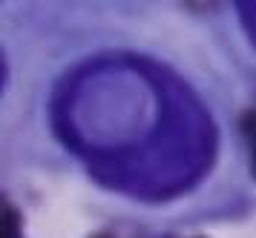
\includegraphics[height=80pt]{backdp/incl1.png}
  \end{subfigure}
  \hspace{0.1cm}
  \begin{subfigure}[t]{0.225\textwidth}
    \centering
    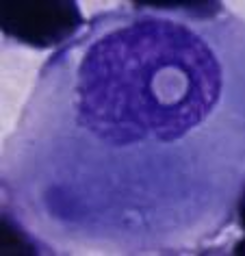
\includegraphics[height=80pt]{backdp/incl2.png}
  \end{subfigure}
  \hspace{0.1cm}
  \begin{subfigure}[t]{0.225\textwidth}
    \centering
    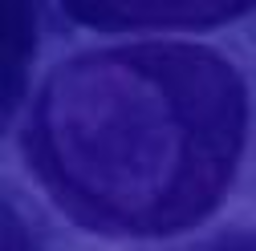
\includegraphics[height=80pt]{backdp/incl3.png}
  \end{subfigure}
  \hspace{0.1cm}
  \begin{subfigure}[t]{0.225\textwidth}
    \centering
    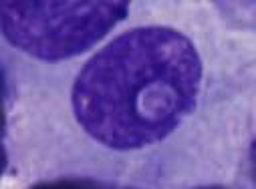
\includegraphics[height=80pt]{backdp/incl4.png}
  \end{subfigure}
  \caption{Example of cells with an intranuclear inclusion from thyroid nodule \acrshort{fnab} smears.}
  \label{fig:backdp:thyroid_inclusion}
\end{figure}

\begin{figure}
  \centering
  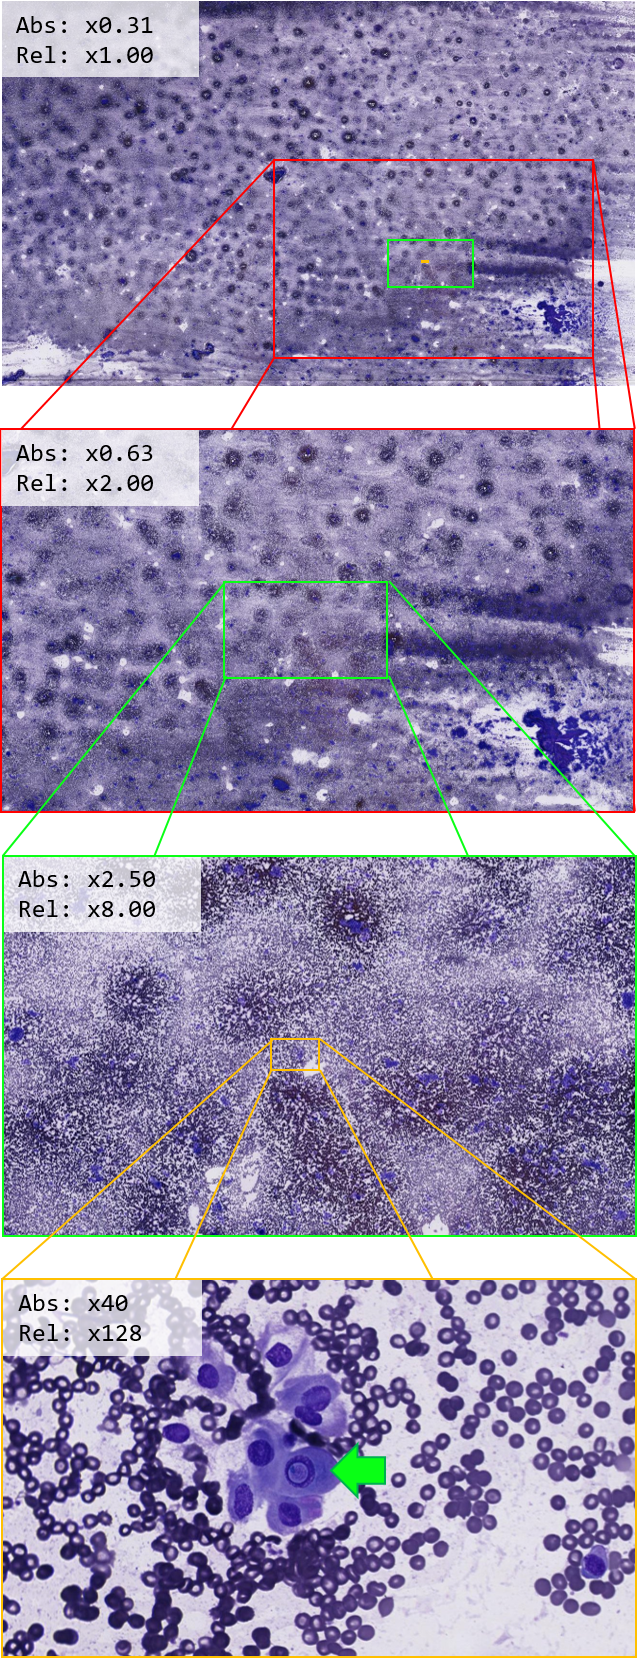
\includegraphics[height=21cm]{backdp/thyroid_needle_haystack.png}
  \caption{Views of an intracellular inclusion at different zoom levels. In the top left corner of each image are the absolute and relative magnifications.}
  \label{fig:backdp:thyroid_needle_haystack}
\end{figure}


\section{Computational pathology and machine learning}
\label{sec:backdp:ml}

Digital pathology has opened the way for the application of \acrlong{ml} to automate analysis and diagnosis. Albeit promising, the application of \acrlong{ml} remains challenging for various reasons. In this section, we discuss some of these challenges then present some techniques that can be used, if not to overcome them, at least to alleviate them.

%  in Sections \ref{ssec:backdp:dataleakage} and \ref{ssec:backdp:datascarcity}

\subsection{Data leakage}
\label{ssec:backdp:dataleakage}

In Section \ref{ssec:backml:modelselinpractice}, we introduced the notion of data leakage that occurs when samples in different splits of a dataset are not independent from each other. Data leakage usually results in poor evaluation of the generalization performance, leading to a poor choice of hyperparameters. Obviously, this should be avoided at all cost especially when the prediction of this model impacts the patient diagnosis and treatment. It is worth noting that data leakage is considered an important obstacle for the application of \acrlong{ml} in biology and medicine in general, not only in \acrlong{dp} \cite{ching2018opportunities}. 

In \acrlong{dp}, data leakage can occur in many, sometimes subtle, ways. Therefore, learning pipelines should be built carefully. One important potential source of data leakage is due to the fact that a whole-slide image does not only convey information about the tissue it contains but also about the slide preparation process (see Section \ref{sec:backdp:wsi}). For instance, staining solutions decay over time. Therefore, the staining intensity can reflect whether the sample has been dipped in a recently-changed or an heavily-used staining bath. When staining is performed manually, the intensity might also reflect the identity of the technician who performed the staining operation. Indeed, some technicians might dip slides for a little longer than others resulting in a stronger intensity. When a dataset is built by different laboratories, the origin of a slide is traceable due to differences in the slide preparation processes between sites. 

These slide idiosyncracies are harmless as long as they are not correlated with the learning problem target. Whereas it might seem unlikely to happen, some simple though unfortunate choices can lead to correlation. For instance, supposing a problem of malignancy assessment, if one laboratory provides all the healthy samples and another all the malignant samples, there is significant risk that the learning algorithm would exploit the differences resulting from the preparation processes. This would obviously lead to poor generalization when the model will be applied to slides coming from another laboratory for instance. 
%This could occur similarly if malignant and healthy slides are provided by the same laboratory but the former are prepared in the morning and the latter in the afternoon.

The slide preparation process is not the only culprit for data leakage. Another possible source occurs at the patient level. \citeauthor{bussola2021ai} \cite{bussola2021ai} have empirically studied patient-wise and random dataset splitting strategies. They have shown that overfitting and data leakage indeed occur when splitting samples randomly.

% {test score worse for patient wise splitting than for tile wise splitting in the article. That's unexpected.}

In general, it is difficult to completely prevent data leakage as one does not always have control over the whole \acrshort{wsi} generation process. However, good practices surely help reducing the problem to an acceptable minimum. A detailed list of guidelines and good practices to reduce the risk of data leakage can be found in \cite{maree2017need}. This includes collecting data as representative as possible of the different variations that could naturally occur during the generation process. For model evaluation and selection, splitting the dataset into subsets should be performed considering the characteristics of the samples that could correlate with the target (\ie patient, laboratory, technician, staining, equipement, time of the day/week, \etc.).

\subsection{About annotations}
\label{ssec:backdp:conceptannotation}

Annotations are important to train \acrlong{ml} models in a supervised manner. They provide information to the algorithm that can adapt the model to fit more accurately the target data. An annotation typically links two elements: an annotation construct and a semantic information. 

An annotation construct concerns the format of the annotation. For instance, in classification, the annotation is a label usually encoded as an integer. For object detection, a common construct is the bounding box framing an object of interest. In image segmentation, the construct is often a hand-drawn polygon covering all pixels belonging to a structure of interest. The semantic information links an annotation to the semantic of the tackled problem and is necessary to differentiate one annotation from another. For instance, in the case of tissue segmentation, the semantic information would be the type of tissue delineated by the hand-drawn polygon (\eg adipose or conjonctive tissue, tumor, metastase).

When it comes to annotating a \acrshort{wsi}s dataset, the level of annotation must also be considered. Indeed, annotation can be performed at slide, region or cellular level. The combination of annotation construct, semantic information and level are an important choice in an annotation project and must be chosen carefully to match the target application and fit the allotted budget \cite{wahab2022semantic}. Indeed, some constructs are more time consuming and therefore expensive to obtain than others (\eg hand-drawn polygons at the cellular level). The cost of annotation is a challenge for \acrlong{cpath} and is one of the causes of data scarcity which is discussed in the next section. 

\subsection{Data scarcity}
\label{ssec:backdp:datascarcity}
% and imperfect annotations

As introduced in Section \ref{ssec:backml:sl}, \textit{data scarcity} refers to a context where data is lacking which usually hampers the performance of \acrlong{ml} methods, especially \acrlong{dl}. Data scarcity is often cited as one of the major challenges in \acrlong{cpath} \cite{tizhoosh2018artificial,litjens2017survey,robertson2018digital,komura2018machine}. A misconception would be to consider that data simply do not exist in a sufficient quantity. Indeed, hospitals and research institutes have accumulated a significant amount of data in different formats over the years (imaging, text, \etc.). What makes \acrlong{cpath} but also the whole field of medical and biological image analysis a data scarce domain is a combination of factors preventing these data to be usable for \acrlong{ml} in a straightforward way.

Many successes in the application of machine and \acrlong{dl} to natural images problems were made possible by the availability of numerous large and exhaustively annotated datasets. For instance, the ImageNet classification dataset features 1000 fine-grained classes for 1.2 million images (see Figure \ref{fig:backdp:illusimagenet}) and has been a key element in \acrlong{dl} innovations since AlexNet. Another example is \acrfirstit{coco} by Microsoft \cite{lin2014microsoft}, a large-scale dataset for segmentation, detection and captioning (\ie assigning a descriptive sentence to an image). It contains more than 200k images annotated with fine segmentation masks over objects from 91 distinct categories (\ie humans, furniture, animals, \etc.). It counts more than 800k unique annotated instances of these categories. Initially published by Google in 2016, the most recent iteration of Open Images Dataset \cite{kuznetsova2020open} contains approximately 9.2 million images each annotated with one or more labels from 19.8k concepts for a total of 30 million image-level labels. JFT-3B is an unpublished dataset from Google introduced in \cite{zhai2106scaling} that contains 3 billion images with noisy labels from a hierarchy of 30k items.

\begin{figure}
  \centering
  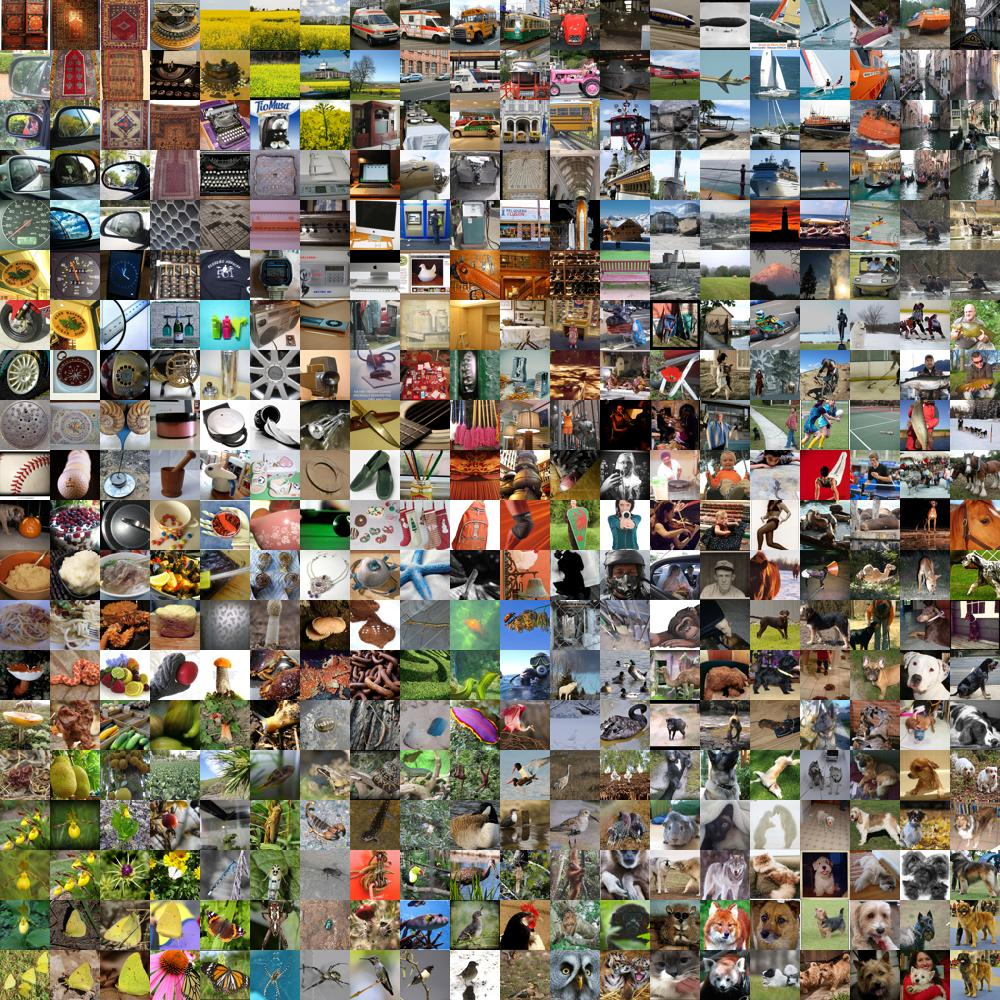
\includegraphics[width=\textwidth]{backdp/illuimagenet.jpg}
  \caption{Samples from ImageNet (source: \cite{img:imagenet}).}
  \label{fig:backdp:illusimagenet}
\end{figure}

Those were only few examples of the plethora of datasets available in the natural image domain. In \acrlong{cpath}, the growing interest for \acrshort{ml}-based solutions has encouraged researchers and practitioners to increasingly share their data and annotations. Although the data scarcity situation is slowly improving, dataset size, versatility and variety are still subpar compared to the natural image domain.

\subsubsection{A mini-review of Grand Challenge pathology datasets from 2021}
\label{sssec:backdp:grandchallenge}

\begin{table}
  \centering
  \footnotesize
  \begin{tabular}{|ccc|ccccccc|}
    \hline
    \multicolumn{3}{|c|}{Challenge} & \# \acrshort{wsi} & \# \acrshort{roi} & \acrshort{roi} size & Crowd & AI-assist. & Task & \# targ. \\
    \hline
    \multirow{3}{*}{\cite{vanrijthoven2021tiger}} & \multirow{3}{*}{TIGER} & tils & 82 & / &  / & yes & yes & REG & $r \in \left[1, 100\right]$\\
    & & rois & 195 & 2032 & $<$ 1.5k $\times$ 1.5k & no & no & SEG & 7\\
    & & bulk & 93 & / & / & no & no & SEG & 2 \\
    \hdashline
    \cite{graham2021conic} & \multicolumn{2}{c|}{CoNiC} & / & 4981 & 256 $\times$ 256 & no & yes & \acrshort{seg}, \acrshort{clf} & 6 \\
    \cite{aubreville2021mitosis} & \multicolumn{2}{c|}{MIDOG 2021} & 50 & 200 & $<$ 5k $\times$ 5k & no & yes & \acrshort{det}, \acrshort{cnt} & 2 \\
    \cite{xu2021predicting} & \multicolumn{2}{c|}{BCNB} & 1058 & / & / & no & no & \acrshort{clf} & 16$^{(1)}$ \\
    \cite{han2021multilayer} & \multicolumn{2}{c|}{WSSS4LUAD} & 87 & 10k & $<$ 300 $\times$ 300 & no & no & \acrshort{clf} & 2\\
    \cite{amgad2019structured} & \multicolumn{2}{c|}{BCSS} & / & 151 & $<$ 7k $\times$ 10k & no & no & \acrshort{seg} & 7\\
    \cite{amgad2021nucls} & \multicolumn{2}{c|}{NuCLS} &  / & 3944 & $<$ 300 $\times$ 300 & yes & yes & \acrshort{seg}, \acrshort{det} & 12 \\
    \cite{kang2021paip} & \multicolumn{2}{c|}{PAIP 2021} & 150 & / & / & no & no & \acrshort{seg}$^{(2)}$ & 4 \\
    \hline
  \end{tabular}
  \caption{List of challenges published in 2021 with the ``histology'' modality on the Grand Challenge website. The ``Crowd'' and 
  ``AI-assist.'' columns relate to the annotation process and how it was performed. The former indicates whether or not non-pathologists 
  were involved in the process (\ie \textit{yes} for crowdsourcing). The latter indicates whether or not the annotation process involved 
  some kind of AI assistance. The ``\# targ.'' indicates the number of target categories/classes of the underlying \acrlong{ml} problem. REG, 
  CLF, SEG, CNT and DET respectively stand for regression, classification, segmentation, counting and detection. $(1)$ The BCNB challenge proposes 6 different classification tasks each with up to 4 classes (for a total of 16 classes). $(2)$ The expected output is not a  classical segmentation mask but rather the boundary of the structure of interest.}
  \label{tab:backdp:datascarcity-grandchallenge}
\end{table}

\begin{figure}
  \centering
  \begin{subfigure}{0.30\textwidth}
    \centering
    % roi-level-annotations/tissue-cells/images/TC_S01_P000183_C0001_B101_[112201, 88004, 113409, 89133].png
    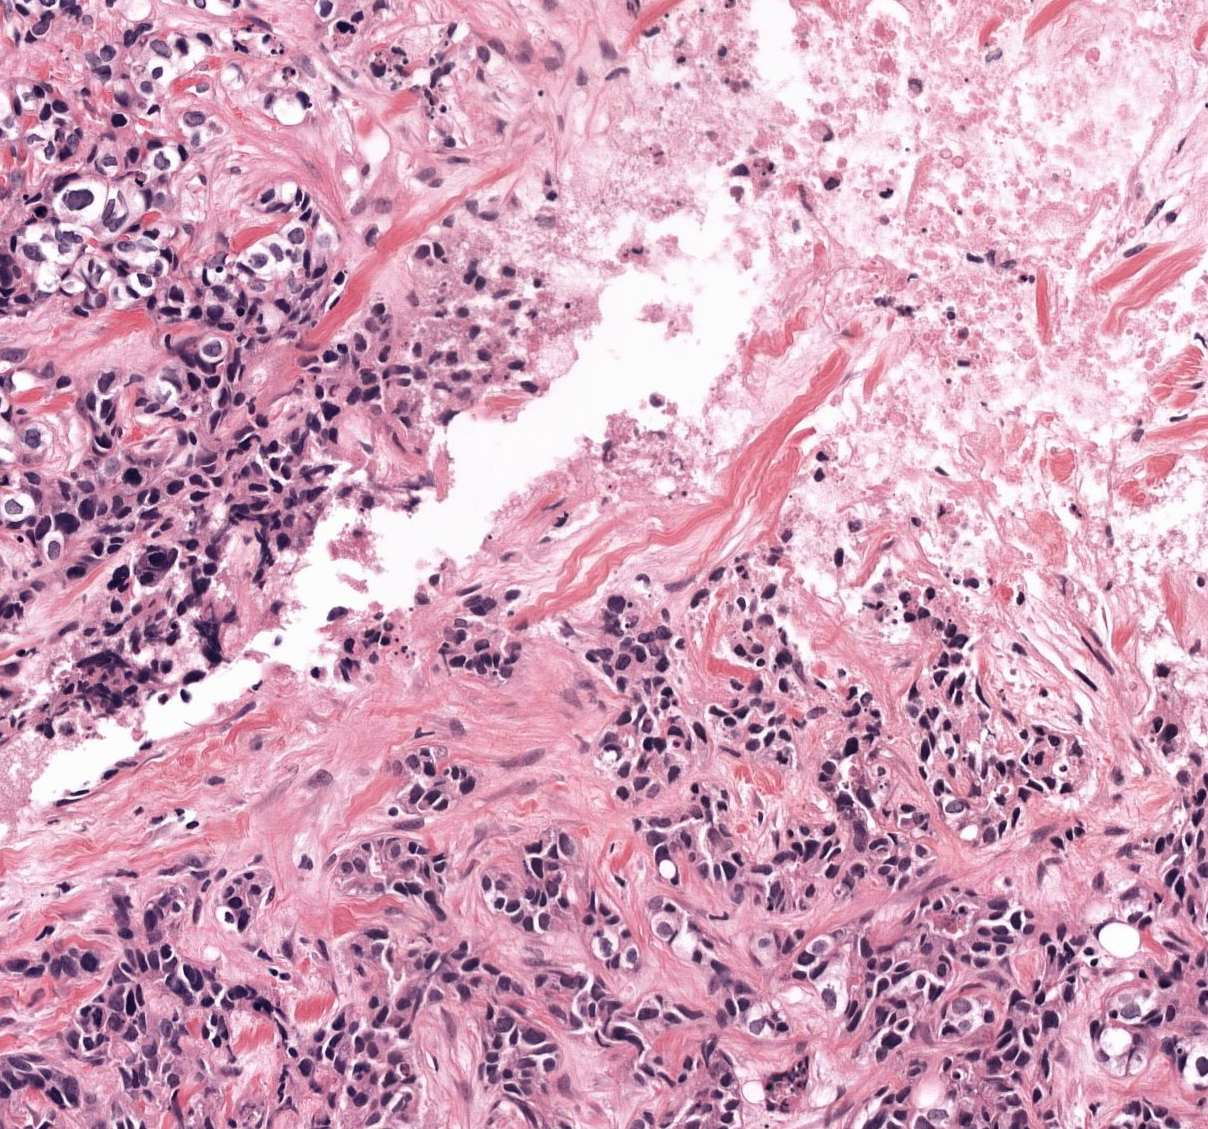
\includegraphics[width=\textwidth]{backdp/tiger_sample.png}
    \caption{TIGER}
    \label{sfig:backdp:challenge_sample:tiger}
  \end{subfigure}
  \begin{subfigure}{0.30\textwidth}
    \centering
    % Lizard_Image1/consep_1.png
    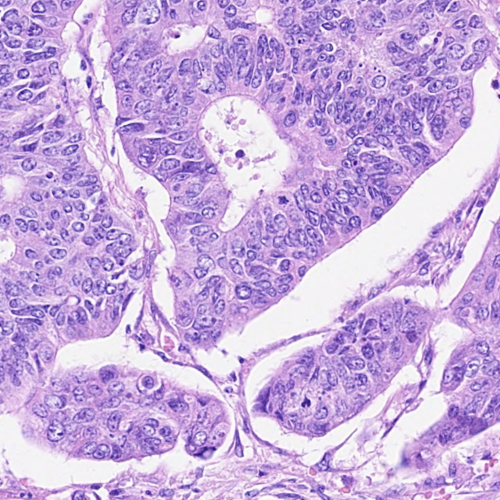
\includegraphics[width=\textwidth]{backdp/lizard_sample.png}
    \caption{CoNiC (Lizard dataset)}
    \label{sfig:backdp:challenge_sample:conic}
  \end{subfigure} 
  \begin{subfigure}{0.30\textwidth}
    \centering
    % 200.tiff
    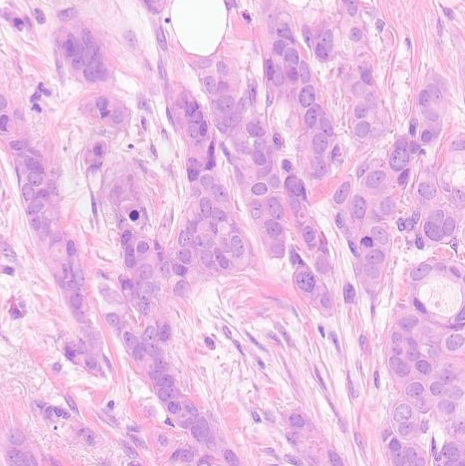
\includegraphics[width=\textwidth]{backdp/midog_sample.png}
    \caption{MIDOG 2021}
    \label{sfig:backdp:challenge_sample:midog}
  \end{subfigure}\\

  \begin{subfigure}{0.30\textwidth}
    \centering
    % 1058.jpg
    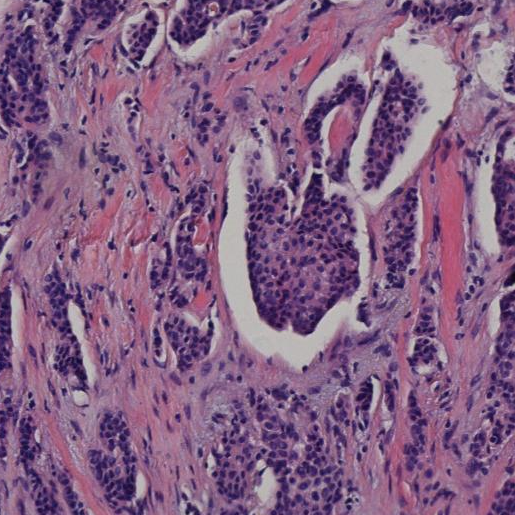
\includegraphics[width=\textwidth]{backdp/bcnb_sample.png}
    \caption{BCNB}
    \label{sfig:backdp:challenge_sample:bcnb}
  \end{subfigure}
  \begin{subfigure}{0.30\textwidth}
    \centering
    % train -> 436219-7159-50847-[1, 1, 0].png 
    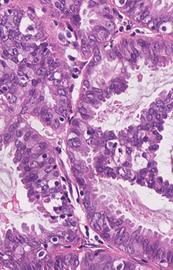
\includegraphics[rotate=90,width=\textwidth]{backdp/wsss4luad_sample.png}
    \caption{WSSS4LUAD}
    \label{sfig:backdp:challenge_sample:wsss4luad}
  \end{subfigure}
  \begin{subfigure}{0.30\textwidth}
    \centering
    % TCGA-A2-A0YM-01Z-00-DX1.A48B4C96-2CC5-464C-98B7-F0F92AE56533.svs
    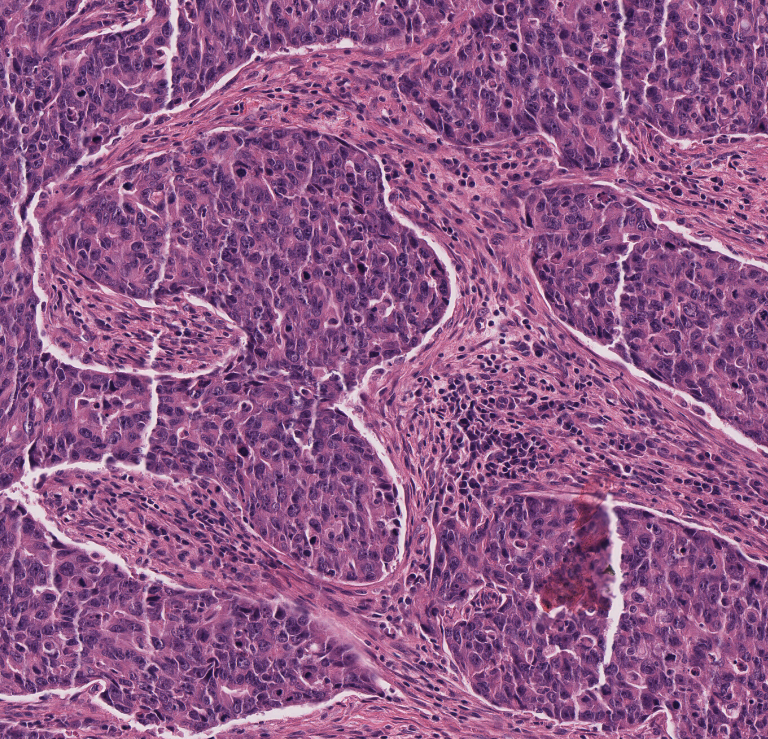
\includegraphics[width=\textwidth]{backdp/bcss_sample.png}
    \caption{BCSS}
    \label{sfig:backdp:challenge_sample:bcss}
  \end{subfigure} \\

  \begin{subfigure}{0.30\textwidth}
    \centering
    % rgbs_colorNormalized/TCGA-S3-AA10-DX1_xmin43039_ymin23986_MPP-0.2500.png
    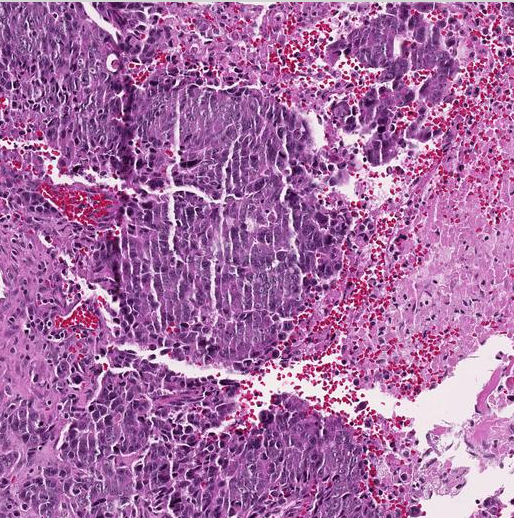
\includegraphics[height=0.22\textheight]{backdp/nucls_sample.png}
    \caption{NuCLS}
    \label{sfig:backdp:challenge_sample:nucls}
  \end{subfigure}
  \begin{subfigure}{0.48\textwidth}
    \centering
    % Col_PNI2021chall_train_0017.svs
    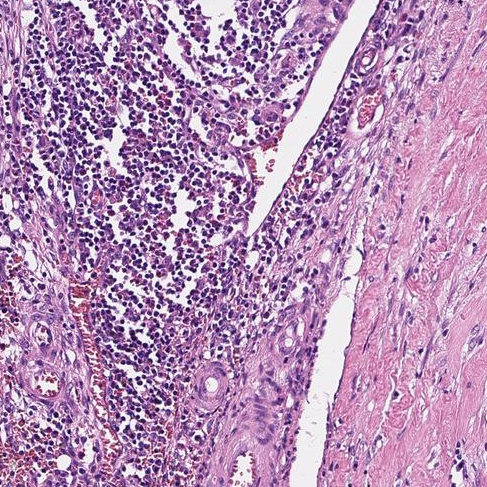
\includegraphics[height=0.22\textheight]{backdp/paip21_sample.png}
    \caption{PAIP 2021}
    \label{sfig:backdp:challenge_sample:paip2021}
  \end{subfigure} 
  \caption{Samples from the Grand Challenge datasets of our mini-review.}
  \label{fig:backp:samples_challenges}
\end{figure}

In order to illustrate this point, we performed a search on the Grand Challenge website \cite{grandchallenge}, a popular platform which runs \acrlong{ml} challenges related to biomedical images, each challenge coming with an open-access dataset. We searched for \textit{histology} challenges published in 2021 and found 8 results (see Table \ref{tab:backdp:datascarcity-grandchallenge} for a brief description of relevant aspects and Figure \ref{fig:backp:samples_challenges} for selected samples of these datasets).

A first observation is that, whether the dataset is a set of \acrshort{wsi} or \textit{\acrlong{roi}s} (\acrshort{roi}), the number of provided images is several orders of magnitude below the number of images available in natural image datasets. It can be argued that the dimensions of \acrshort{wsi} and \acrshort{roi} images in \acrlong{dp} datasets is significantly larger that natural images (\eg average image size in ImageNet is 469 $\times$ 387 pixels, the largest of the 151 \acrshort{roi} of BCSS reaches approximately 7k $\times$ 10k pixels), however this must be put in perspective in relation to the prediction task. For instance, hundreds of \acrshort{wsi}s represent a very large amount of raw data (\eg few terabytes) but, when the target task is whole-slide classification, this only amounts to a hundred of annotated samples which is significantly fewer compared to ImageNet or others and can be considered a rather small sample size from a \acrshort{ml} perspective.  

Beyond the size of datasets, it is interesting to note that most prediction tasks in \acrlong{dp} only feature few classes (at most 12 in our Grand Challenge sample). It is common to encounter tasks presented as binary (\eg malignant \vs benign) even though it is often a simplification of the underlying biological or medical problem. Datasets with a large variety of classes have shown to be effective for learning efficient models on natural images. Therefore, on this matter, \acrlong{cpath} is still lagging behind significantly. 

It is also interesting to consider how these datasets were built. Among them, four datasets use internal data acquired and annotated specifically for the challenge (PAIP 2021, MIDOG 2021, BCNB, BCSS), two of them mix both internal and external data (TIGER, WSSS4LUAD) and the last two use exclusively data from external sources (CoNiC, NuCLS). Regarding the use of external data, it either means that external \acrshort{wsi} were imported and annotated for the challenge or that data from other datasets were combined together. For instance, the CoNiC challenge is based on the Lizard dataset \cite{graham2021lizard} which combines data from the \acrfirstit{tcga} \cite{weinstein2013cancer}, PanNuke \cite{gamper2019pannuke}, CRAG \cite{graham2019mild}, CoNSeP \cite{graham2019hover}, GlaS \cite{sirinukunwattana2017gland} and DigestPath \cite{li2019signet}. The \acrshort{tcga} is an open platform gathering various data related to cancer genomic including a little more than 30k \acrlong{wsi}s, making it one of the largest open databases of \acrshort{wsi} to date. It is no surprise that, over the years, many datasets have been built using the \acrshort{tcga} as one of their sources. This also includes WSSS4LUAD, TIGER and NuCLS from our Grand Challenge sample. Interestingly, one of the components of Lizard, PanNuke has also been built from \acrfirst{tcga} and three external datasets of which two were built on top of the same platform (MoNuSeg \cite{kumar2019multi} and CMP17 \cite{vu2019methods}). Although it raises the question of the risk of data leakage, assembling existing datasets to form a larger one certainly helps fighting data scarcity.

\subsubsection{Causes}
\label{sssec:backdp:ds-causes}

The mini-review performed in the previous section was not aimed at being a thorough evaluation of \acrshort{dp} datasets characteristics. It rather serves as a way to highlight different consequences of data scarcity in the field: small dataset size, lack of variety and versatility, \etc. The scarcity in \acrlong{dp} is caused by a combination of factors.  

One of the main causes of scarcity is the cost of the annotation process. Pathology is not a simple subject and slide evaluation requires years of training and experience. Whereas classifying pictures into object categories can be done by mostly anyone, creating a ground truth \acrlong{dp} dataset requires trained pathologists for whom time is a precious and expensive resource. Therefore, annotation cost in \acrlong{dp} is significantly higher compared to the natural image domain. This is aggravated by the fact that disagreement between pathologists is not uncommon and quality ground truth usually requires confronting and aggregating annotations by several experts. 


Privacy and ethical concerns also play a role. Indeed, medical data is sensitive and cannot be shared without patient consent, rightfully so, preventing data to be made available for \acrlong{ml}. Privacy might incur additional costs as it might be necessary to keep track where data records have been used, for instance, in the context of the European \acrfirst{gdpr}. Indeed, in case a patient revokes his data sharing agreement, under the right-to-be-forgotten, models might have to be re-trained \cite{humerick2017taking}. Overall, it can discourage researchers and practitioners to make their data available. 

The use of data-hungry \acrlong{dl} algorithms does not help and is aggravated by the need for a dataset to contain enough samples to account for the variability incurred by the slides content and preparation process. 

% On another front, complexity and duration of the slide preparation process makes it more difficult to produce new \acrshort{wsi} than natural images like pictures which can be captured with any smartphone nowadays. Currently, slide preparation is definitely not a bottleneck as opposed to labeling but could become one if  throughput of quality annotations.

\subsubsection{How to work around data scarcity ?}
\label{sssec:backdp:ds-solutions}

The causes of data scarcity are numerous and it remains a challenge for \acrlong{cpath} but the situation is evolving positively. 

Nowadays, there exist annotation strategies which allow to cut the cost per annotation and therefore produce larger datasets given the same budget. These strategies include crowdsourcing through citizen science \cite{peplow2016citizen} or the intervention of medical students (\eg NuCLS dataset). These approaches obviously require either supervision by pathologists or more annotations per image to average out the inaccuracies (or even both) but these are in general less expensive than direct annotation by trained pathologists. It is also possible to indirectly reduce the annotation cost by reducing the time spent per annotation. One way of achieving that is to use the \acrshort{ai} to assist experts and accelerate the annotation process (see NuCLS, CoNiC, MIDOG 2021 from our Grand Challenge sample) \cite{chai2020human}. A weak but fast algorithm could for instance suggest cell boundaries. The annotator could then correct the boundaries if necessary which is less time-consuming than drawing them from scratch. The use of dedicated and intuitive user interface with efficient drawing tools can also help in that regard.  

If annotating new data is not an option, it is also possible to combat data scarcity by the use of existing external data and proper computational methods \cite{van2019strategies}. There exist several open resources for \acrlong{dp} \cite{maree2019open} providing access to slides and annotations. We have already introduced \acrshort{tcga} which provides access to a spectacular amount of 30k \acrshort{wsi}. The Camelyon dataset introduced in Section \ref{ssec:backdp:analysis_camelyon} contains 1399 \acrshort{wsi} of which 209 were annotated at full resolution with detailed hand-drawn contours of all metastases. This is one of the largest most-precisely annotated datasets in the field to date. The Lizard dataset (subject of the CoNiC challenge) contains almost 500k segmented nuclei all labeled into one of 6 classes. Some promising projects are also ongoing such as Bigpicture \cite{moulin2021imi} of which the goals are to ``\textit{create the first European, ethically compliant, and quality-controlled whole slide imaging platform, in which both large-scale data and AI algorithms will exist}''. This project aims at having the same impact on \acrlong{cpath} as ImageNet had on the natural image domain by constructing a database of millions of digital slides.

Sometimes the lack of data is such that the dataset is not representative enough of the different variations that could occur in a realistic context. The impact of this issue can be alleviated during the training process directly with an ad-hoc data augmentation procedure that would automatically generate the kind of variations that can be expected (\eg staining intensity, deformation, \etc.). Data normalization during pre-processing such as stain normalization can also help in that regard \cite{kang2021stainnet, runz2021normalization, zhao2022restainnet}.

Regarding the computational methods, there exist machine and \acrlong{dl} algorithms which can make use of external or sparse data. We explore some of them in the thesis and present related works in the following sections. 

\subsection{Transfer learning}
\label{ssec:backdp:tl}

Transfer learning (see Sections \ref{ssec:backml:transfer} and \ref{ssec:backml:dl:deeptransfer}) is one of the most popular techniques for tackling data scarcity. In this section, we explore how deep transfer learning was applied to biomedical images. Some of the first applications were reported in \cite{bar2015chest,ciompi2015automatic,van2015off} for pulmonary nodule detection in chest x-rays and \acrshort{ct}-scans using Decaf and OverFeat (feature extractors based on ImageNet and AlexNet) as feature extractors. While those works have revealed the potential of deep transfer learning in that field, the performances were not significantly better than those of previous methods. \citeauthor{ravishankar2016understanding} \cite{ravishankar2016understanding} compared the performance of a pre-trained AlexNet-based CaffeNet \cite{jia2014caffe} to well-established computer vision like \acrfirstit{hog} \cite{mcconnell1986method} and found the former to outperform the latter.

Later, as new ImageNet architectures emerged, their transfer potential from ImageNet was also evaluated on various biomedical imaging tasks. \citeauthor{antony2016quantifying} \cite{antony2016quantifying} evaluated the use of fine-tuning and feature extraction of different architectures including VGG16 for quantifying knee osteoarthritis severity on radiography images. \citeauthor{kieffer2017convolutional} \cite{kieffer2017convolutional} compared training from scratch to both feature extraction and fine-tuning for classification and retrieval of pathology images using InceptionV3 and VGG16. \citeauthor{shin2016deep} \cite{shin2016deep} studied the interest of transfer of different architectures including GoogLeNet and AlexNet for thoracoabdominal lymph node detection and interstitial lung disease classification. Some of these works and others \cite{ponzio2019dealing, tajbakhsh2016convolutional} have shown that transfer learning usually yielded better performance than training neural networks from scratch.

As introduced earlier, some works have shown that transfer learning is likely to provide better performance when the source and target tasks are close \cite{yosinski2014transferable} or if the source task includes the target domain \cite{mensink2021factors}. This implies that pre-training models on pathology data directly is a sound approach although it requires a significant amount of source data to make a proper source task. This was confirmed in several contributions.

For instance, \citeauthor{khan2019improving} \cite{khan2019improving} pre-train an InceptionV3 network on a custom dataset generated from Camelyon16 and then transfer the resulting model to a prostate cancer classification task. They show that their pre-trained model outperforms both training from scratch and using an ImageNet pre-trained model. \citeauthor{medela2019few} \cite{medela2019few} also use transfer learning between two pathology tasks but rather than following a classical supervised pre-training approach, they adopt a self-supervised algorithm by training a siamese network to distinguish between different parts of colorectal tissues. The network is then transferred as a feature extractor on the target task (tumor classification). \citeauthor{shang2019and} \cite{shang2019and} use several datasets (including some unrelated to their target task such as \textit{Dogs vs. cats}) and compare ImageNet and domain-specific pre-training in order to tackle colonoscopy image classification. They also show that pre-training on domain-specific data yield superior performance compared to using ImageNet. \citeauthor{kraus2017automated} \cite{kraus2017automated} train a custom deep neural architecture, DeepLoc, for classifying protein subcellular localization in budding yeast. Then, they assess the transferability of their pre-trained DeepLoc by fine-tuning it on different image sets, including unseen classes, and show that the pre-training is indeed beneficial.

\subsection{Multi-task learning}
\label{ssec:backdp:mtl}

Multi-task learning (see Section \ref{ssec:backml:mtl} and \ref{ssec:backml:dl:deepmultitask}) has been applied to medical imaging. \citeauthor{samala2017multi} \cite{samala2017multi} jointly train a classifier on three mammography image datasets (digitized screen-film and digital mammograms) and compare it to single-task training and transfer learning. They show that a multi-task trained network generalizes better than a single-task one. \citeauthor{zhang2016deep} \cite{zhang2016deep} use transfer and multi-task learning to derive image features from Drosophila gene expression. MTL has also been applied more specifically to \acrlong{cpath}. \citeauthor{pan2018multi} \cite{pan2018multi} apply MTL for breast cancer classification by using a classification loss and a verification loss. The role of the latter is to ensure that features produced by the network differ for images of different classes. \citeauthor{arvaniti2018coupling} \cite{arvaniti2018coupling} use both weak and strong supervision at once to classify prostate cancer. \citeauthor{shang2019and} \cite{shang2019and} evaluate multi-task learning which is the best performing approach on their target task. However, they suggest that more experiments would have to be carried out to assess whether their conclusions are generalizable.

\subsection{Self-training and weakly supervised learning}
\label{ssec:backdp:st}

We have introduced self-training in Sections \ref{ssec:backml:inbetween} and \ref{ssec:backml:dl:selftraining}. It is not surprising that self-training has also been applied to medical image tasks to combat data scarcity \cite{tajbakhsh2020embracing, peng2021medical} and to \acrlong{cpath} in particular. Most works in this domain currently treat with image classification \cite{peikari2018cluster, su2019local, koohbanani2021self, jaiswal2019semi, shaw2020teacher} but detection and segmentation have also been explored. \citeauthor{li2018based} \cite{li2018based} combine weakly-supervised learning and self-training to predict per-pixel Gleason score across entire WSIs. \citeauthor{li2019signet} \cite{li2019signet} build a signet ring cell detector using self-training. To mitigate the impact of erroneous pseudo-label, their approach features a cooperative training step where two models are trained on the pseudo-labels generated by one another during the previous round. Self-training has also been applied to segmentation for other image modalities. To segment cardiac MR images, \citeauthor{bai2017semi} \cite{bai2017semi} propose a self-training approach to train a segmentation architecture. In particular, the teacher and student are the same model and the student is not reset between training rounds. Additionally, they apply a \acrfirstit{crf} to refine the model predictions on the unlabeled images. \citeauthor{fan2020inf} \cite{fan2020inf} focus on lung infection segmentation in the context of the COVID-19 pandemic. Their approach features a self-training protocol where at every training round, they pseudo-label $K$ new unlabeled images which will be added to the learning set for the next round. 

Semi-supervised literature also concerns the use of imperfect data which relates more to \acrlong{wsl}. This approach has also been explored for biomedical tasks. \citeauthor{wolny2021sparse} \cite{wolny2021sparse} learn from sparse instance segmentation masks using their sparse single object loss which combines an instance-based loss and an embedding consistency loss. They also evaluate their method on two microscopy images datasets. \citeauthor{bokhorst2018learning} \cite{bokhorst2018learning} segment tissues from colorectal cancer patients into 13 classes representing different types of tissues. Their dataset is composed of both exhaustively- and sparsely-labeled images. During training, they apply a weight map to tune and balance the contribution of individual pixels to the loss. The masks ignore unannotated pixels. On the \acrshort{glas} dataset \cite{sirinukunwattana2017gland}, \citeauthor{foucart2019snow} \cite{foucart2019snow} study how performance of different segmentation methods including semi- and weakly-supervised techniques are impacted by dataset imperfections (\eg deformation, missing annotations, \etc.). They show that fully supervised approaches are able to cope with noise up to a certain level but quickly degrade after that and that semi-supervised methods are able to partially recover from these degradations.  

\section{Wrapping up}

This chapter introduced the domains of digital and \acrlong{cpath} and gave an overview of different challenges encountered in these fields: high variability in the slide preparation and scanning processes, lack of annotated data, high data volumes, \etc. These challenges for sure have slowed down the advances in automated image analysis techniques but the situation is evolving quickly as many initiatives are under way to change that. Given the high practical relevance of automated tools in the domain, one can only expect that the interest in \acrlong{cpath} will continue to grow and envision a future where new image acquisition and analysis techniques will not only revolutionize image analysis itself but also the pathology and diagnosis workflow as a whole. In this thesis, we explore transfer, multi-task and semi-supervised learning in order to tackle \acrlong{cpath} problems and attempt to work around data scarcity.